\documentclass{article}
% \VignettePackage{dapc}
% \VignetteIndexEntry{An introduction to the adegenet package}

\usepackage{graphicx}
\usepackage[colorlinks=true,urlcolor=blue]{hyperref}
\usepackage{array}
\usepackage{color}

\usepackage[utf8]{inputenc} % for UTF-8/single quotes from sQuote()


% for bold symbols in mathmode
\usepackage{bm}

\newcommand{\R}{\mathbb{R}}
\newcommand{\beq}{\begin{equation}}
\newcommand{\eeq}{\end{equation}}
\newcommand{\m}[1]{\mathbf{#1}}



\newcommand{\code}[1]{{{\tt #1}}}
\title{An introduction to \textit{adegenet} 1.3-0}
\author{Thibaut Jombart}
\date{\today}




\sloppy
\hyphenpenalty 10000


\usepackage{Sweave}
\begin{document}





\definecolor{Soutput}{rgb}{0,0,0.56}
\definecolor{Sinput}{rgb}{0.56,0,0}
\DefineVerbatimEnvironment{Sinput}{Verbatim}
{formatcom={\color{Sinput}},fontsize=\footnotesize, baselinestretch=0.75}
\DefineVerbatimEnvironment{Soutput}{Verbatim}
{formatcom={\color{Soutput}},fontsize=\footnotesize, baselinestretch=0.75}

\color{black}

\maketitle

\begin{abstract}
  This vignette provides an introductory tutorial to the \textit{adegenet} package \cite{tjart05}
  for the R software \cite{np145}. This package implements tools to handle, analyse and simulate
  genetic data.  Originally developped for multiallelic, codominant markers such as microsatellites,
  \textit{adegenet} now also handles dominant markers, allows for any ploidy in the data, and
  implements the most memory-efficient storage and handling of genome-wide SNP data. This vignette
  introduces basic functionalities of the package. Other vignettes are dedicated to specific topics
  (see Introduction below).
\end{abstract}


\newpage
\tableofcontents




\newpage
%%%%%%%%%%%%%%%%%%%%%%%%%%%%%%%%%%%%%%%%%%%%%%%%%%
%%%%%%%%%%%%%%%%%%%%%%%%%%%%%%%%%%%%%%%%%%%%%%%%%%
\section{Introduction}
%%%%%%%%%%%%%%%%%%%%%%%%%%%%%%%%%%%%%%%%%%%%%%%%%%
%%%%%%%%%%%%%%%%%%%%%%%%%%%%%%%%%%%%%%%%%%%%%%%%%%
This tutorial introduces some basic functionalities of the \textit{adegenet} package for R \cite{np145}.
The purpose of this package is to provide tools for handling, analysing and simulating genetic
markers data, with an emphasis on multivariate approaches and exploratory methods.
Standard multivariate analyses are implemented in the \textit{ade4} package \cite{tj548}, of which
\textit{adegenet} was originally an extension.
However, the package has since grown methods of its own such as the Discriminant Analysis of
Principal Components (DAPC, \cite{tjart19}), the spatial Principal Components Analysis (sPCA,
\cite{tjart04}), or the \textit{SeqTrack} algorithm \cite{tjart20}.


Data can be imported from a wide range of formats, including those of
popular software (GENETIX, STRUCTURE, Fstat, Genepop), or from simple dataframes of genotypes.
Polymorphic sites can be extracted from both nucleotide and amino-acid sequences, with special
methods for handling genome-wide SNPs data with maximum efficiency.
\\

In this tutorial, we first introduce the \texttt{genind} and \texttt{genpop} classes used to store
multiallelic markers (respectively for individuals and populations), and then show how to extract
information from these objects using a variety of tools.  Other vignettes are dedicated to some
specific topics:
\begin{itemize}
\item sPCA: type \texttt{vignette("adegenet-spca",package='adegenet')}
\item DAPC: type \texttt{vignette("adegenet-dapc",package='adegenet')} in R to access this vignette.
\item genome-wide SNPs handling and analysis: type \texttt{vignette("adegenet-genomics",package='adegenet')}
\end{itemize}




\newpage
%%%%%%%%%%%%%%%%%%%%%%%%%%%%%%%%%%%%%%%%%%%%%%%%%%
%%%%%%%%%%%%%%%%%%%%%%%%%%%%%%%%%%%%%%%%%%%%%%%%%%
\section{Getting started}
%%%%%%%%%%%%%%%%%%%%%%%%%%%%%%%%%%%%%%%%%%%%%%%%%%
%%%%%%%%%%%%%%%%%%%%%%%%%%%%%%%%%%%%%%%%%%%%%%%%%%


%%%%%%%%%%%%%%%%%%%%%%%%%%
\subsection{Installing the package}
%%%%%%%%%%%%%%%%%%%%%%%%%%
Before going further, we shall make sure that \textit{adegenet} is weel installed
on the computer.
Current version of the package is 1.3-0.
Make sure you have a recent version ($\geq 2.13.0$) of R by typing:
\begin{Schunk}
\begin{Sinput}
> R.version.string
\end{Sinput}
\begin{Soutput}
[1] "R version 2.13.0 (2011-04-13)"
\end{Soutput}
\end{Schunk}

Then, install \textit{adegenet} with dependencies using:
\begin{Schunk}
\begin{Sinput}
> install.packages("adegenet", dep = TRUE)
\end{Sinput}
\end{Schunk}
This only installs packages on CRAN.
However, some functions in \textit{adegenet} also use \textit{graph}, developped on Bioconductor, an
alternative package repository.
To install \textit{graph}, type:
\begin{Schunk}
\begin{Sinput}
> source("http://bioconductor.org/biocLite.R")
> biocLite("graph")
\end{Sinput}
\end{Schunk}

We can now load the package using:
\begin{Schunk}
\begin{Sinput}
> library(adegenet)
\end{Sinput}
\end{Schunk}

\noindent You can make sure that the right version of the package is installed using:
\begin{Schunk}
\begin{Sinput}
> packageDescription("adegenet", fields = "Version")
\end{Sinput}
\begin{Soutput}
[1] "1.3-0"
\end{Soutput}
\end{Schunk}
\textit{adegenet} version should read 1.3-0.




%%%%%%%%%%%%%%%%%%%%%%%%%%
\subsection{Getting help}
%%%%%%%%%%%%%%%%%%%%%%%%%%
There are several ways of getting information about R in general, or about
\textit{adegenet} in particular.
The function \texttt{help.search} is used to look for help on a given topic.
For instance:
\begin{Schunk}
\begin{Sinput}
> help.search("Hardy-Weinberg")
\end{Sinput}
\end{Schunk}
replies that there is a function \texttt{HWE.test.genind} in the
\textit{adegenet} package, other similar functions in \textit{genetics} and \textit{pegas}.
To get help for a given function, use \texttt{?foo} where `foo' is the
function of interest.
For instance (quotes can be removed):
\begin{Schunk}
\begin{Sinput}
> `?`(spca)
\end{Sinput}
\end{Schunk}
will open up the manpage of the spatial principal component analysis \cite{tjart04}.
At the end of a manpage, an `example' section often shows how to use a function.
This can be copied and pasted to the console, or directly executed
from the console using \texttt{example}.
For further questions concerning R, the function \texttt{RSiteSearch}
is a powerful tool for making online researches using keywords in R's archives (mailing
lists and manpages).
\\


\textit{adegenet} has a few extra documentation sources.
Information can be found from the website
(\url{http://adegenet.r-forge.r-project.org/}), in the `documents'
section, including tutorial and a manual which includes all
manpages of the package, and a dedicated mailing list with searchable archives.
To open the website from R, use:
\begin{Schunk}
\begin{Sinput}
> adegenetWeb()
\end{Sinput}
\end{Schunk}
The same can be done for tutorials, using \texttt{adegenetTutorial} (see
manpage to choose the tutorial to open).
Alternatively, one can use \texttt{vignette}, for which \texttt{adegenetTutorial} is merely a wrapper.

You will also find a listing of the main functions of the package typing:
\begin{Schunk}
\begin{Sinput}
> `?`(adegenet)
\end{Sinput}
\end{Schunk}

Note that you can also browse help pages as html pages, using:
\begin{Schunk}
\begin{Sinput}
> help.start()
\end{Sinput}
\end{Schunk}
To go to the \textit{adegenet} page, click `packages', `adegenet', and
`adegenet-package'.
\\


Lastly, several mailing lists are available to find different kinds of
information on R; to name a few:
\begin{itemize}
\item adegenet forum
  (\url{https://lists.r-forge.r-project.org/cgi-bin/mailman/listinfo/adegenet-forum}):
  adegenet and multivariate analysis of genetic markers
\item R-help (\url{https://stat.ethz.ch/mailman/listinfo/r-help}):
  general questions about R
\item R-sig-genetics
  (\url{https://stat.ethz.ch/mailman/listinfo/r-sig-genetics}):
  genetics in R
\item R-sig-phylo
  (\url{https://stat.ethz.ch/mailman/listinfo/r-sig-phylo}):
  phylogenetics in R
\end{itemize}






\newpage
%%%%%%%%%%%%%%%%%%%%%%%%%%%%%%%%%%%%%%%%%%%%%%%%%%
%%%%%%%%%%%%%%%%%%%%%%%%%%%%%%%%%%%%%%%%%%%%%%%%%%
\section{Object classes}
%%%%%%%%%%%%%%%%%%%%%%%%%%%%%%%%%%%%%%%%%%%%%%%%%%
%%%%%%%%%%%%%%%%%%%%%%%%%%%%%%%%%%%%%%%%%%%%%%%%%%
Two classes of objects are used for storing genetic marker data, depending on the level at which the genetic information is considered:
\texttt{genind} is used for individual genotypes, whereas \texttt{genpop} is used for alleles numbers counted by populations.
Note that the term 'population', here and later, is employed in a broad sense: it simply refers to any grouping of individuals.
The specific class \texttt{genlight} is used for storing large genome-wide SNPs data.
See \textit{adegenet-genomics} vignette for more information.

%%%%%%%%%%%%%%%%%%%%%%%%%%%%%%%%%%%%%%%%%%%%%%%%%%
\subsection{genind objects}
%%%%%%%%%%%%%%%%%%%%%%%%%%%%%%%%%%%%%%%%%%%%%%%%%%
These objects can be obtained by reading data files from other software,
from a \texttt{data.frame} of genotypes, by conversion from a table of
allelic frequencies, or even from aligned DNA or proteic sequences (see 'importing data').
\begin{Schunk}
\begin{Sinput}
> data(nancycats)
> is.genind(nancycats)
\end{Sinput}
\begin{Soutput}
[1] TRUE
\end{Soutput}
\begin{Sinput}
> nancycats
\end{Sinput}
\begin{Soutput}
   #####################
   ### Genind object ### 
   #####################
- genotypes of individuals - 

S4 class:  genind
@call: genind(tab = truenames(nancycats)$tab, pop = truenames(nancycats)$pop)

@tab:  237 x 108 matrix of genotypes

@ind.names: vector of  237 individual names
@loc.names: vector of  9 locus names
@loc.nall: number of alleles per locus
@loc.fac: locus factor for the  108 columns of @tab
@all.names: list of  9 components yielding allele names for each locus
@ploidy:  2
@type:  codom

Optionnal contents: 
@pop:  factor giving the population of each individual
@pop.names:  factor giving the population of each individual

@other: a list containing: xy 
\end{Soutput}
\end{Schunk}
A \texttt{genind} object is formal S4 object with several slots,
accessed using the '\texttt{@}' operator (see \texttt{class?genind}).
Note that the '\texttt{\$}' was also implemented for adegenet objects,
so that slots can be accessed as if they were components of a list.
\\

The structure of \texttt{genind} objects is described by:
\begin{Schunk}
\begin{Sinput}
> getClassDef("genind")
\end{Sinput}
\begin{Soutput}
Class "genind" [package "adegenet"]

Slots:
                                                                       
Name:           tab    loc.names      loc.fac     loc.nall    all.names
Class:       matrix    character factorOrNULL     intOrNum   listOrNULL
                                                                       
Name:          call    ind.names          pop    pop.names       ploidy
Class:   callOrNULL    character factorOrNULL   charOrNULL      integer
                                
Name:          type        other
Class:    character   listOrNULL

Extends: "gen", "indInfo"
\end{Soutput}
\end{Schunk}

The slightly cryptic output of this function means that \texttt{genind} objects possess the following slots:
\begin{itemize}
  \item \texttt{tab}: a table of relative allele frequencies (individuals in rows, alleles in columns).
  \item \texttt{loc.names}: a vector of labels for the loci.
  \item \texttt{loc.fac}: a factor indicating which columns in \texttt{@tab} correspond to which marker.
  \item \texttt{loc.nall}: the number of alleles in each marker.
  \item \texttt{all.names}: a vector of labels for the alleles.
  \item \texttt{ind.names}:  a vector of labels for the individuals.
  \item \texttt{pop}: a factor storing group membership of the individuals.
  \item \texttt{pop.names}: labels used for populations.
  \item \texttt{ploidy}: the ploidy level of the genome.
  \item \texttt{type}: a character string indicating whether the marker is codominant
    (\texttt{codom}) or presence/absence ('\texttt{PA}').
  \item \texttt{other}: a list storing optional information.
  \item \texttt{call}: the matched call, i.e. command used to create the object.
\end{itemize}
Slots can be accessed using '\texttt{@}' or '\texttt{\$}', although in some cases it is more
convenient to use accessors (i.e. function which return specific content of the object) than
accessing the slot directly (see section 'Using accessors').
\\

The main slot in \texttt{genind} is the table of allelic frequencies of individuals (in rows) for
every alleles in every loci stored in \texttt{@tab}.
Being frequencies, data sum to one per locus, giving the score of 1 for an homozygote and 0.5 for an heterozygote.
The particular case of presence/absence data will is described in an
ad-hoc section (see 'Handling presence/absence data').
For instance:
\begin{Schunk}
\begin{Sinput}
> nancycats$tab[10:18, 1:10]
\end{Sinput}
\begin{Soutput}
    L1.01 L1.02 L1.03 L1.04 L1.05 L1.06 L1.07 L1.08 L1.09 L1.10
010     0     0     0     0     0   0.0   0.0   0.0   1.0   0.0
011     0     0     0     0     0   0.0   0.0   0.0   0.0   0.5
012     0     0     0     0     0   0.5   0.0   0.5   0.0   0.0
013     0     0     0     0     0   0.5   0.0   0.5   0.0   0.0
014     0     0     0     0     0   0.0   0.0   1.0   0.0   0.0
015     0     0     0     0     0   0.0   0.5   0.0   0.5   0.0
016     0     0     0     0     0   0.5   0.0   0.0   0.5   0.0
017     0     0     0     0     0   0.5   0.0   0.5   0.0   0.0
018     0     0     0     0     0   0.5   0.0   0.0   0.5   0.0
\end{Soutput}
\end{Schunk}
Individual '010' is an homozygote for the allele 09 at locus 1, while '018' is an heterozygote with alleles 06 and 09.
As user-defined labels are not always valid (for instance, they can
be duplicated), generic labels are used for individuals, markers, alleles and eventually population.
The true names are stored in the object (components \texttt{\$[...].names} where ... can be 'ind', 'loc', 'all' or 'pop').
For instance :
\begin{Schunk}
\begin{Sinput}
> nancycats$loc.names
\end{Sinput}
\begin{Soutput}
     L1      L2      L3      L4      L5      L6      L7      L8      L9 
 "fca8" "fca23" "fca43" "fca45" "fca77" "fca78" "fca90" "fca96" "fca37" 
\end{Soutput}
\end{Schunk}
gives the true marker names, and
\begin{Schunk}
\begin{Sinput}
> nancycats$all.names[[3]]
\end{Sinput}
\begin{Soutput}
   01    02    03    04    05    06    07    08    09    10 
"133" "135" "137" "139" "141" "143" "145" "147" "149" "157" 
\end{Soutput}
\end{Schunk}
gives the allele names for marker 3.


\noindent The slot 'ploidy' is an integer giving the level of ploidy
of the considered organisms (defaults to 2).
This parameter is essential, in particular when switching from
individual frequencies (\texttt{genind} object) to allele counts per
populations (\texttt{genpop}).

\noindent
The slot 'type' describes the type of marker used: codominant ('codom', e.g. microsatellites) or presence/absence ('PA', e.g. AFLP).
By default, adegenet considers that markers are codominant.
Note that actual handling of presence/absence markers has been made available since version 1.2-3.
See the dedicated section for more information about presence/absence markers.
\\


Optional content can are also be stored within the object.
The slot \texttt{@other} is a list that can include any additional information.
The optional slot \texttt{@pop} (a factor giving a grouping of individuals) is particular in that the behaviour of many functions will check automatically for it and behave accordingly.
In fact, each time an argument 'pop' is required by a function, it is first seeked in \texttt{@pop}.
For instance, using the function \texttt{genind2genpop} to convert \texttt{nancycats} to a \texttt{genpop} object, there is no need to give a 'pop' argument as it exists in the \texttt{genind} object:
\begin{Schunk}
\begin{Sinput}
> table(nancycats$pop)
\end{Sinput}
\begin{Soutput}
P01 P02 P03 P04 P05 P06 P07 P08 P09 P10 P11 P12 P13 P14 P15 P16 P17 
 10  22  12  23  15  11  14  10   9  11  20  14  13  17  11  12  13 
\end{Soutput}
\begin{Sinput}
> catpop <- genind2genpop(nancycats)
\end{Sinput}
\begin{Soutput}
 Converting data from a genind to a genpop object... 

...done.
\end{Soutput}
\begin{Sinput}
> catpop
\end{Sinput}
\begin{Soutput}
       #####################
       ### Genpop object ### 
       #####################
- Alleles counts for populations - 

S4 class:  genpop
@call: genind2genpop(x = nancycats)

@tab:  17 x 108 matrix of alleles counts

@pop.names: vector of  17 population names
@loc.names: vector of  9 locus names
@loc.nall: number of alleles per locus
@loc.fac: locus factor for the  108 columns of @tab
@all.names: list of  9 components yielding allele names for each locus
@ploidy:  2
@type:  codom

@other: a list containing: xy 
\end{Soutput}
\end{Schunk}
Other additional components can be stored (like here, spatial coordinates of populations in \$xy) but will not be passed during any conversion (\texttt{catpop} has no \$other\$xy).
\\

Finally, a \texttt{genind} object generally contains its matched call, \textit{i.e.} the instruction that created it.
This is not the case, however, for objects loaded using \texttt{data}.
When call is available, it can be used to regenerate an object.
\begin{Schunk}
\begin{Sinput}
> obj <- read.genetix(system.file("files/nancycats.gtx", package = "adegenet"))
\end{Sinput}
\begin{Soutput}
 Converting data from GENETIX to a genind object... 

...done.
\end{Soutput}
\begin{Sinput}
> obj$call
\end{Sinput}
\begin{Soutput}
read.genetix(file = system.file("files/nancycats.gtx", package = "adegenet"))
\end{Soutput}
\begin{Sinput}
> toto <- eval(obj$call)
\end{Sinput}
\begin{Soutput}
 Converting data from GENETIX to a genind object... 

...done.
\end{Soutput}
\begin{Sinput}
> identical(obj, toto)
\end{Sinput}
\begin{Soutput}
[1] TRUE
\end{Soutput}
\end{Schunk}


%%%%%%%%%%%%%%%%%%%%%%%%%%%%%%%%%%%%%%%%%%%%%%%%%%
\subsection{genpop objects}
%%%%%%%%%%%%%%%%%%%%%%%%%%%%%%%%%%%%%%%%%%%%%%%%%%
We use the previously built \texttt{genpop} object:
\begin{Schunk}
\begin{Sinput}
> catpop
\end{Sinput}
\begin{Soutput}
       #####################
       ### Genpop object ### 
       #####################
- Alleles counts for populations - 

S4 class:  genpop
@call: genind2genpop(x = nancycats)

@tab:  17 x 108 matrix of alleles counts

@pop.names: vector of  17 population names
@loc.names: vector of  9 locus names
@loc.nall: number of alleles per locus
@loc.fac: locus factor for the  108 columns of @tab
@all.names: list of  9 components yielding allele names for each locus
@ploidy:  2
@type:  codom

@other: a list containing: xy 
\end{Soutput}
\begin{Sinput}
> is.genpop(catpop)
\end{Sinput}
\begin{Soutput}
[1] TRUE
\end{Soutput}
\begin{Sinput}
> catpop$tab[1:5, 1:10]
\end{Sinput}
\begin{Soutput}
   L1.01 L1.02 L1.03 L1.04 L1.05 L1.06 L1.07 L1.08 L1.09 L1.10
01     0     0     0     0     0     0     0     2     9     1
02     0     0     0     0     0    10     9     8    14     2
03     0     0     0     4     0     0     0     0     1    10
04     0     0     0     3     0     0     0     1     7    17
05     0     0     0     1     0     0     0     0     7    10
\end{Soutput}
\end{Schunk}
The matrix \$tab contains alleles counts per population (here, cat colonies).
These objects are otherwise very similar to \texttt{genind} in their
structure, and possess generic names, true names, the matched call and
an \texttt{@other} slot:
\begin{Schunk}
\begin{Sinput}
> getClassDef("genpop")
\end{Sinput}
\begin{Soutput}
Class "genpop" [package "adegenet"]

Slots:
                                                                       
Name:           tab    loc.names      loc.fac     loc.nall    all.names
Class:       matrix    character factorOrNULL     intOrNum   listOrNULL
                                                                       
Name:          call    pop.names       ploidy         type        other
Class:   callOrNULL    character      integer    character   listOrNULL

Extends: "gen", "popInfo"
\end{Soutput}
\end{Schunk}



%%%%%%%%%%%%%%%%%%%%%%%%%%%%%%%%%%%%%%%%%%%%%%%%%%
\subsection{Using accessors}
%%%%%%%%%%%%%%%%%%%%%%%%%%%%%%%%%%%%%%%%%%%%%%%%%%
One advantage of formal (S4) classes is that they allow for interacting simply with possibly complex objects.
This is made possible by using accessors, i.e. functions that extract information from an object,
rather than accessing the slots directly.
Another advantage of this approach is that as long as accessors remain identical on the user's
side, the internal structure of an object may change from one release to another without generating
errors in old scripts.
Although \texttt{genind} and \texttt{genpop} objects are fairly simple, we recommend using accessors whenever possible
to access their content.
\\

Available accessors are:
\begin{itemize}
  \item \texttt{nInd}: returns the number of individuals in the object; only for \texttt{genind}.
  \item \texttt{nLoc}: returns the number of loci (SNPs).
  \item \texttt{indNames}$^{\dagger}$: returns/sets labels for individuals; only for \texttt{genind}.
  \item \texttt{locNames}$^{\dagger}$: returns/sets labels for loci (SNPs).
  \item \texttt{alleles}$^{\dagger}$: returns/sets alleles.
  \item \texttt{ploidy}$^{\dagger}$: returns/sets ploidy of the individuals.
  \item \texttt{pop}$^{\dagger}$: returns/sets a factor grouping individuals; only for \texttt{genind}.
  \item \texttt{other}$^{\dagger}$: returns/sets misc information stored as a list.
\end{itemize}
where $^{\dagger}$ indicates that a replacement method is available using \texttt{<-}; for instance:
\begin{Schunk}
\begin{Sinput}
> head(indNames(nancycats), 10)
\end{Sinput}
\begin{Soutput}
   001    002    003    004    005    006    007    008    009    010 
"N215" "N216" "N217" "N218" "N219" "N220" "N221" "N222" "N223" "N224" 
\end{Soutput}
\begin{Sinput}
> indNames(nancycats) <- paste("cat", 1:nInd(nancycats), sep = ".")
> head(indNames(nancycats), 10)
\end{Sinput}
\begin{Soutput}
     001      002      003      004      005      006      007      008 
 "cat.1"  "cat.2"  "cat.3"  "cat.4"  "cat.5"  "cat.6"  "cat.7"  "cat.8" 
     009      010 
 "cat.9" "cat.10" 
\end{Soutput}
\end{Schunk}

Some accessors such as \texttt{locNames} may have specific options:
\begin{Schunk}
\begin{Sinput}
> locNames(nancycats)
\end{Sinput}
\begin{Soutput}
     L1      L2      L3      L4      L5      L6      L7      L8      L9 
 "fca8" "fca23" "fca43" "fca45" "fca77" "fca78" "fca90" "fca96" "fca37" 
\end{Soutput}
\begin{Sinput}
> head(locNames(nancycats, withAlleles = TRUE), 10)
\end{Sinput}
\begin{Soutput}
 [1] "fca8.117" "fca8.119" "fca8.121" "fca8.123" "fca8.127" "fca8.129"
 [7] "fca8.131" "fca8.133" "fca8.135" "fca8.137"
\end{Soutput}
\end{Schunk}

\noindent The slot 'pop' can be retrieved and set using \texttt{pop}:
\begin{Schunk}
\begin{Sinput}
> obj <- nancycats[sample(1:50, 10)]
> pop(obj)
\end{Sinput}
\begin{Soutput}
 [1] 2 2 2 4 2 3 3 3 3 1
Levels: 2 4 3 1
\end{Soutput}
\begin{Sinput}
> pop(obj) <- rep("newPop", 10)
> pop(obj)
\end{Sinput}
\begin{Soutput}
 [1] newPop newPop newPop newPop newPop newPop newPop newPop newPop newPop
Levels: newPop
\end{Soutput}
\end{Schunk}
An additional advantage of using accessors is they are most of the time safer. For instance,
\texttt{pop<-} will check the length of the new group membership vector against the data, and
complain if there is a mismatch.






\newpage
%%%%%%%%%%%%%%%%%%%%%%%%%%%%%%%%%%%%%%%%%%%%%%%%%%
%%%%%%%%%%%%%%%%%%%%%%%%%%%%%%%%%%%%%%%%%%%%%%%%%%
\section{Importing/exporting data}
%%%%%%%%%%%%%%%%%%%%%%%%%%%%%%%%%%%%%%%%%%%%%%%%%%
%%%%%%%%%%%%%%%%%%%%%%%%%%%%%%%%%%%%%%%%%%%%%%%%%%


%%%%%%%%%%%%%%%%%%%%%%%%%%%%%%%%%%%%%%%%%%%%%%%%%%
\subsection{Importing data from GENETIX, STRUCTURE, FSTAT, Genepop}
%%%%%%%%%%%%%%%%%%%%%%%%%%%%%%%%%%%%%%%%%%%%%%%%%%

Data can be read from the software GENETIX (.gtx), STRUCTURE (.str or
.stru), FSTAT (.dat) and Genepop (.gen) files, using the corresponding
\texttt{read} function: \texttt{read.genetix},  \texttt{read.structure},
\texttt{read.fstat}, and  \texttt{read.genepop}.
These functions take as main argument the path (as a string character) to an input file, and produce a \texttt{genind} object.
Alternatively, one can use the function \texttt{import2genind} which detects a file format from its extension and uses the appropriate routine.
For instance:
\begin{Schunk}
\begin{Sinput}
> obj1 <- read.genetix(system.file("files/nancycats.gtx", package = "adegenet"))
\end{Sinput}
\begin{Soutput}
 Converting data from GENETIX to a genind object... 

...done.
\end{Soutput}
\begin{Sinput}
> obj2 <- import2genind(system.file("files/nancycats.gtx", package = "adegenet"))
\end{Sinput}
\begin{Soutput}
 Converting data from GENETIX to a genind object... 

...done.
\end{Soutput}
\begin{Sinput}
> all.equal(obj1, obj2)
\end{Sinput}
\begin{Soutput}
[1] "Attributes: < Component 2: target, current do not match when deparsed >"
\end{Soutput}
\end{Schunk}

\noindent The only difference between \texttt{obj1} and \texttt{obj2} is
their call (which is normal as they were obtained from different
command lines).




%%%%%%%%%%%%%%%%%%%%%%%%%%%%%%%%%%%%%%%%%%%%%%%%%%
\subsection{Importing data from other software}
%%%%%%%%%%%%%%%%%%%%%%%%%%%%%%%%%%%%%%%%%%%%%%%%%%
Genetic markers data can most of the time be stored as a table with individuals in row and markers
in column, where each entry is a character string coding the alleles possessed at one locus.
Such data are easily imported into R as a \texttt{data.frame}, using for instance \texttt{read.table}
for text files or \texttt{read.csv} for comma-separated text files.
Then, the obtained \texttt{data.frame} can be converted into a \texttt{genind} object using \texttt{df2genind}.
\\

There are only a few pre-requisite the data should meet for this conversion to be possible. The
easiest and clearest way of coding data is using a separator between alleles. For instance,
"80/78'', "80|78", or "80,78'' are different ways of coding a genotype at a microsatellite locus
with alleles '80' and 78".
Note that for haploid data, no separator shall be used.
As a consequence, SNP data should consist of the raw nucleotides.
The only contraint when using a separator is that the same separator is used in all the
dataset. There are no contraints as to i) the type of separator used or ii) the ploidy of the data.
These parameters can be set in \texttt{df2genind} through arguments 'sep' and 'ploidy', respectively.
\\

Alternatively, no separator may be used provided a fixed number of characters is used to code any allele.
For instance, in a diploid organism, "0101" is an homozygote 1/1 while "1209" is a heterozygote
12/09 in a two-character per allele coding scheme.
In a tetraploid system with one character per allele, "1209" will be understood as 1/2/0/9.

Here, we provide an example using randomly generated tetraploid data.
\begin{Schunk}
\begin{Sinput}
> temp <- lapply(1:30, function(i) sample(0:9, 4, replace = TRUE))
> temp <- sapply(temp, paste, collapse = "")
> temp <- matrix(temp, nrow = 10, dimnames = list(paste("ind", 
+     1:10), paste("loc", 1:3)))
> temp
\end{Sinput}
\begin{Soutput}
       loc 1  loc 2  loc 3 
ind 1  "0652" "7624" "1903"
ind 2  "6442" "4143" "6414"
ind 3  "9753" "5886" "5226"
ind 4  "3754" "3336" "6535"
ind 5  "2245" "5586" "9674"
ind 6  "7438" "1568" "5184"
ind 7  "8488" "8386" "5272"
ind 8  "1293" "8206" "1952"
ind 9  "9159" "6431" "9701"
ind 10 "8507" "5481" "0490"
\end{Soutput}
\begin{Sinput}
> obj <- df2genind(temp, ploidy = 4, sep = "")
> obj
\end{Sinput}
\begin{Soutput}
   #####################
   ### Genind object ### 
   #####################
- genotypes of individuals - 

S4 class:  genind
@call: df2genind(X = temp, sep = "", ploidy = 4)

@tab:  10 x 29 matrix of genotypes

@ind.names: vector of  10 individual names
@loc.names: vector of  3 locus names
@loc.nall: number of alleles per locus
@loc.fac: locus factor for the  29 columns of @tab
@all.names: list of  3 components yielding allele names for each locus
@ploidy:  4
@type:  codom

Optionnal contents: 
@pop:  - empty -
@pop.names:  - empty -

@other: - empty -
\end{Soutput}
\end{Schunk}

\noindent \texttt{obj} is a \texttt{genind} containing the same information, but recoded as a matrix of allele
frequencies (\texttt{\$tab} slot).





%%%%%%%%%%%%%%%%%%%%%%%%%%%%%%%%%%%%%%%%%%%%%%%%%%
\subsection{Handling presence/absence data}
%%%%%%%%%%%%%%%%%%%%%%%%%%%%%%%%%%%%%%%%%%%%%%%%%%
Adegenet was primarly suited to handle codominant, multiallelic markers like microsatellites.
However, dominant binary markers, like AFLP, can be used as well.
In such a case, only presence/absence of alleles can be deduced accurately from
the genotypes.
This has several consequences, like the unability to compute allele frequencies.
Hence, some functionalities in adegenet won't be available for
dominant markers.

From version 1.2-3 of adegenet, the distinction between both types of markers is made by the slot
'type' of genind or genpop objects, which equals "codom" for
codominant markers, and "PA" for presence/absence data.
In the latter case, the 'tab' slot of a genind object no longer contains allele
frequencies, but only presence/absence of alleles in a genotype.
Similarly, the 'tab' slot of a genpop object not longer contains
counts of alleles in the populations; instead, it contains the number
of genotypes in each population possessing at least one copy of the concerned alleles.
Moreover, in the case of presence/absence, the slots 'loc.nall', 'loc.fac', and 'all.names'
become useless, and are thus all set to NULL.
\\


Objects of type 'PA' are otherwise handled like usual (type 'codom')
objects.
Operations that are not available for PA type will issue an appropriate error message.

Here is an example using a toy dataset 'AFLP.txt' that can be downloaded
from the adegenet website, section 'Documentation':
\begin{Schunk}
\begin{Sinput}
> dat <- read.table(system.file("files/AFLP.txt", package = "adegenet"), 
+     header = TRUE)
> dat
\end{Sinput}
\begin{Soutput}
     loc1 loc2 loc3 loc4
indA    1    0    1    1
indB    0    1    1    1
indC    1    1    0    1
indD    0   NA    1   NA
indE    1    1    0    0
indF    1    0    1    1
indG    0    1    1    0
\end{Soutput}
\end{Schunk}
\noindent The function \texttt{df2genind} is used to obtain a genind object:
\begin{Schunk}
\begin{Sinput}
> obj <- genind(dat, ploidy = 1, type = "PA")
> obj
\end{Sinput}
\begin{Soutput}
   #####################
   ### Genind object ### 
   #####################
- genotypes of individuals - 

S4 class:  genind
@call: genind(tab = dat, ploidy = 1, type = "PA")

@tab:  7 x 4 matrix of genotypes

@ind.names: vector of  7 individual names
@loc.names: vector of  4 locus names
@loc.nall: NULL
@loc.fac: NULL
@all.names: NULL
@ploidy:  1
@type:  PA

Optionnal contents: 
@pop:  - empty -
@pop.names:  - empty -

@other: - empty -
\end{Soutput}
\begin{Sinput}
> truenames(obj)
\end{Sinput}
\begin{Soutput}
     loc1 loc2 loc3 loc4
indA    1    0    1    1
indB    0    1    1    1
indC    1    1    0    1
indD    0   NA    1   NA
indE    1    1    0    0
indF    1    0    1    1
indG    0    1    1    0
\end{Soutput}
\end{Schunk}

One can see that for instance, the summary of this object is more simple (no numbers of alleles per locus, no heterozygosity):
\begin{Schunk}
\begin{Sinput}
> pop(obj) <- rep(c("a", "b"), 4:3)
> summary(obj)
\end{Sinput}
\begin{Soutput}
 # Total number of genotypes:  7 

 # Population sample sizes:  
a b 
4 3 

 # Percentage of missing data:  
[1] 7.142857
\end{Soutput}
\end{Schunk}

\noindent But we can still perform basic manipulation, like converting
our object into a genpop:
\begin{Schunk}
\begin{Sinput}
> obj2 <- genind2genpop(obj)
\end{Sinput}
\begin{Soutput}
 Converting data from a genind to a genpop object... 

...done.
\end{Soutput}
\begin{Sinput}
> obj2
\end{Sinput}
\begin{Soutput}
       #####################
       ### Genpop object ### 
       #####################
- Alleles counts for populations - 

S4 class:  genpop
@call: genind2genpop(x = obj)

@tab:  2 x 4 matrix of alleles counts

@pop.names: vector of  2 population names
@loc.names: vector of  4 locus names
@loc.nall: NULL
@loc.fac: NULL
@all.names: NULL
@ploidy:  1
@type:  PA

@other: - empty -
\end{Soutput}
\begin{Sinput}
> obj2@tab
\end{Sinput}
\begin{Soutput}
  L1 L2 L3 L4
1  2  2  3  3
2  2  2  2  1
\end{Soutput}
\end{Schunk}

\noindent To continue with the toy example, we can proceed to a simple PCA.
NAs are first replaced:
\begin{Schunk}
\begin{Sinput}
> objNoNa <- na.replace(obj, met = 0)
\end{Sinput}
\begin{Soutput}
 Replaced 2 missing values 
\end{Soutput}
\begin{Sinput}
> objNoNa@tab
\end{Sinput}
\begin{Soutput}
  L1 L2 L3 L4
1  1  0  1  1
2  0  1  1  1
3  1  1  0  1
4  0  0  1  0
5  1  1  0  0
6  1  0  1  1
7  0  1  1  0
\end{Soutput}
\end{Schunk}

\noindent Now the PCA is performed:
\begin{Schunk}
\begin{Sinput}
> library(ade4)
> pca1 <- dudi.pca(objNoNa, scannf = FALSE, scale = FALSE)
> scatter(pca1)
\end{Sinput}
\end{Schunk}
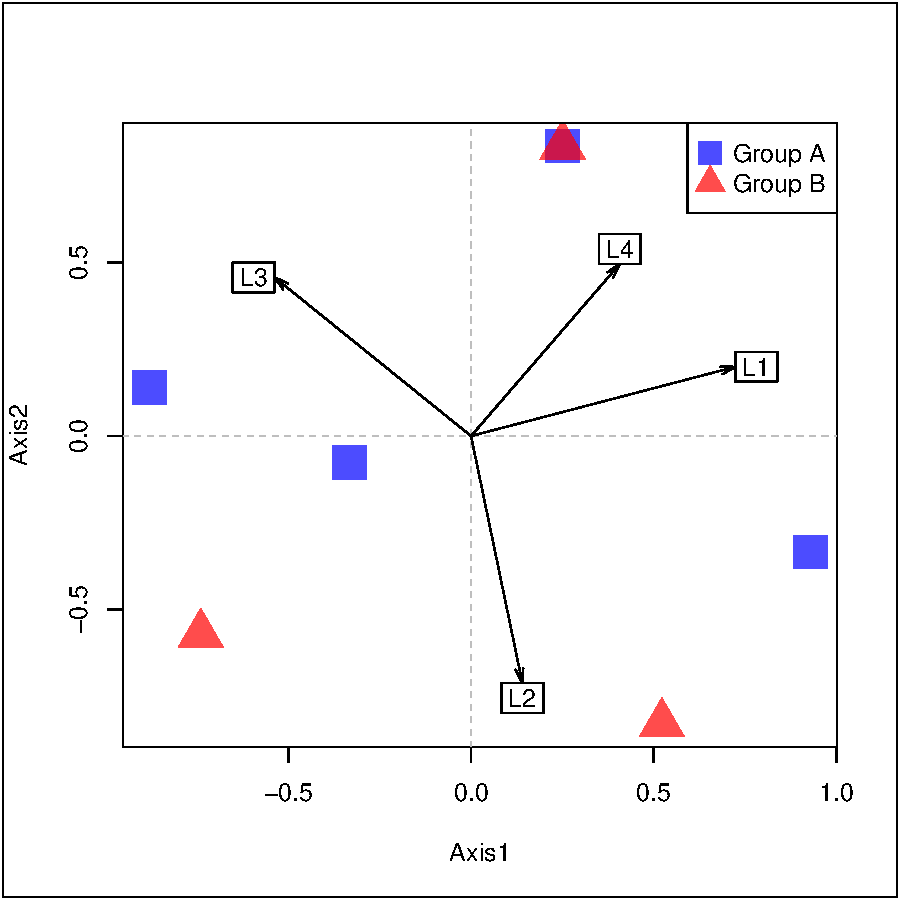
\includegraphics{figs/base-pcaaflp}

\noindent More generally, multivariate analyses from ade4, the sPCA (\texttt{spca}), the
global and local tests (\texttt{global.rtest}, \texttt{local.rtest}), or
the Monmonier's algorithm (\texttt{monmonier}) will work just fine
with presence/absence data.
However, it is clear that the usual Euclidean distance (used in PCA
and sPCA), as well as many other distances, is not as accurate to measure genetic dissimilarity using
presence/absence data as it is when using allele frequencies.
The reason for this is that in presence/absence data, a part of the
information is simply hidden.
For instance, two individuals possessing the same allele will be
considered at the same distance, whether they possess one or more
copies of the allele.
This might be especially problematic in organisms having a high degree
of ploidy.





%%%%%%%%%%%%%%%%%%%%%%%%%%%%%%%%%%%%%%%%%%%%%%%%%%
\subsection{SNPs data}
%%%%%%%%%%%%%%%%%%%%%%%%%%%%%%%%%%%%%%%%%%%%%%%%%%
In adegenet, SNP data can be handled in two different ways.
For relatively small datasets (up to a few thousand SNPs) SNPs can
be handled as other codominant markers such as microsatellites using \texttt{genind} objects.
In the case of genome-wide SNP data (from hundreds of thousands to millions of SNPs),
\texttt{genind} objects are no longer efficient representation of the data.
In this case, we use \texttt{genlight} objects to store and handle information with maximum
efficiency and minimum memory requirements. See the vignette \textit{adegenet-genomics} for more information.
\\

The most convenient way to convert SNPs into a \texttt{genind} is using \texttt{df2genind}, which is
described in the previous section.
Let \texttt{dat} be an input matrix, as can be read into R using \texttt{read.table} or \texttt{read.csv},
with genotypes in row and SNP loci in columns.
\begin{Schunk}
\begin{Sinput}
> dat <- matrix(sample(c("a", "t", "g", "c"), 15, replace = TRUE), 
+     nrow = 3)
> rownames(dat) <- paste("genot.", 1:3)
> colnames(dat) <- 1:5
> dat
\end{Sinput}
\begin{Soutput}
         1   2   3   4   5  
genot. 1 "g" "g" "a" "t" "g"
genot. 2 "g" "c" "g" "g" "c"
genot. 3 "t" "g" "t" "c" "a"
\end{Soutput}
\begin{Sinput}
> obj <- df2genind(dat, ploidy = 1)
> truenames(obj)
\end{Sinput}
\begin{Soutput}
         1.g 1.t 2.c 2.g 3.a 3.g 3.t 4.c 4.g 4.t 5.a 5.c 5.g
genot. 1   1   0   0   1   1   0   0   0   0   1   0   0   1
genot. 2   1   0   1   0   0   1   0   0   1   0   0   1   0
genot. 3   0   1   0   1   0   0   1   1   0   0   1   0   0
\end{Soutput}
\end{Schunk}

\texttt{obj} is a \texttt{genind} containing the SNPs information, which can be used for further
analysis in adegenet.



%%%%%%%%%%%%%%%%%%%%%%%%%%%%%%%%%%%%%%%%%%%%%%%%%%
\subsection{Extracting polymorphism from DNA sequences}
%%%%%%%%%%%%%%%%%%%%%%%%%%%%%%%%%%%%%%%%%%%%%%%%%%
This section only covers the cases of relatively small datasets which can be handled efficiently
using \texttt{genind} objects. For bigger (near full-genomes) datasets, SNPs can be extracted from
\textit{fasta} files into a \texttt{genlight} object using \texttt{fasta2genlight}.
See the vignette \textit{adegenet-genomics} for more information.
\\


DNA sequences can be read into R using the ape package \cite{tj527}, and
imported into adegenet using \texttt{DNAbin2genind}.
There are several ways ape can be used to read in DNA sequences.
The easiest one is reading data from a usual format such as FASTA or Clustal using \texttt{read.dna}.
Other options include reading data directly from GenBank using \texttt{read.GenBank}, or from other
public databases using the seqinr package and transforming the \texttt{alignment} object into a
\texttt{DNAbin} using \texttt{as.DNAbin}.
Here, we illustrate this approach by re-using the example of \texttt{read.GenBank}. A connection to
the internet is required, as sequences are read directly from a distant database.
\begin{Schunk}
\begin{Sinput}
> library(ape)
> ref <- c("U15717", "U15718", "U15719", "U15720", "U15721", "U15722", 
+     "U15723", "U15724")
> myDNA <- read.GenBank(ref)
> myDNA
\end{Sinput}
\begin{Soutput}
8 DNA sequences in binary format stored in a list.

All sequences of same length: 1045 

Labels: U15717 U15718 U15719 U15720 U15721 U15722 ...

Base composition:
    a     c     g     t 
0.267 0.351 0.134 0.247 
\end{Soutput}
\begin{Sinput}
> class(myDNA)
\end{Sinput}
\begin{Soutput}
[1] "DNAbin"
\end{Soutput}
\begin{Sinput}
> summary(myDNA)
\end{Sinput}
\begin{Soutput}
       Length Class  Mode
U15717 1045   DNAbin raw 
U15718 1045   DNAbin raw 
U15719 1045   DNAbin raw 
U15720 1045   DNAbin raw 
U15721 1045   DNAbin raw 
U15722 1045   DNAbin raw 
U15723 1045   DNAbin raw 
U15724 1045   DNAbin raw 
\end{Soutput}
\end{Schunk}
In adegenet, only polymorphic loci are conserved; importing data from a DNA sequence to adegenet
therefore consist in extracting SNPs from the aligned sequences.
This conversion is achieved by \texttt{DNAbin2genind}.
This function allows one to specify a threshold for polymorphism; for instance, one could retain
only SNPs for which the second largest allele frequency is greater than 1\% (using the \texttt{polyThres} argument).
This is achieved using:
\begin{Schunk}
\begin{Sinput}
> obj <- DNAbin2genind(myDNA, polyThres = 0.01)
> obj
\end{Sinput}
\begin{Soutput}
   #####################
   ### Genind object ### 
   #####################
- genotypes of individuals - 

S4 class:  genind
@call: DNAbin2genind(x = myDNA, polyThres = 0.01)

@tab:  8 x 318 matrix of genotypes

@ind.names: vector of  8 individual names
@loc.names: vector of  155 locus names
@loc.nall: number of alleles per locus
@loc.fac: locus factor for the  318 columns of @tab
@all.names: list of  155 components yielding allele names for each locus
@ploidy:  1
@type:  codom

Optionnal contents: 
@pop:  - empty -
@pop.names:  - empty -

@other: - empty -
\end{Soutput}
\end{Schunk}
Here, out of the 1045 nucleotides of the sequences, 318 SNPs where extracted and stored as a
\texttt{genind} object.






%%%%%%%%%%%%%%%%%%%%%%%%%%%%%%%%%%%%%%%%%%%%%%%%%%
\subsection{Extracting polymorphism from proteic sequences}
%%%%%%%%%%%%%%%%%%%%%%%%%%%%%%%%%%%%%%%%%%%%%%%%%%
Alignments of proteic sequences can be exploited in adegenet in the same way as DNA sequences (see
section above).
Alignments are scanned for polymorphic sites, and only those are retained to form a \texttt{genind} object.
Loci correspond to the position of the residue in the alignment, and alleles correspond to the
different amino-acids (AA).
Aligned proteic sequences are stored as objects of class \texttt{alignment} in the \emph{seqinr}
package \cite{np160}.
See \texttt{?as.alignment} for a description of this class.
The function extracting polymorphic sites from \texttt{alignment} objects is \texttt{alignment2genind}

Its use is fairly simple. It is here illustrated using a small dataset of aligned proteic sequences:
\begin{Schunk}
\begin{Sinput}
> library(seqinr)
> mase.res <- read.alignment(file = system.file("sequences/test.mase", 
+     package = "seqinr"), format = "mase")
> mase.res
\end{Sinput}
\begin{Soutput}
$nb
[1] 6

$nam
[1] "Langur" "Baboon" "Human"  "Rat"    "Cow"    "Horse" 

$seq
$seq[[1]]
[1] "-kifercelartlkklgldgykgvslanwvclakwesgynteatnynpgdestdygifqinsrywcnngkpgavdachiscsallqnniadavacakrvvsdqgirawvawrnhcqnkdvsqyvkgcgv-"

$seq[[2]]
[1] "-kifercelartlkrlgldgyrgislanwvclakwesdyntqatnynpgdqstdygifqinshywcndgkpgavnachiscnallqdnitdavacakrvvsdqgirawvawrnhcqnrdvsqyvqgcgv-"

$seq[[3]]
[1] "-kvfercelartlkrlgmdgyrgislanwmclakwesgyntratnynagdrstdygifqinsrywcndgkpgavnachlscsallqdniadavacakrvvrdqgirawvawrnrcqnrdvrqyvqgcgv-"

$seq[[4]]
[1] "-ktyercefartlkrngmsgyygvsladwvclaqhesnyntqarnydpgdqstdygifqinsrywcndgkpraknacgipcsallqdditqaiqcakrvvrdqgirawvawqrhcknrdlsgyirncgv-"

$seq[[5]]
[1] "-kvfercelartlkklgldgykgvslanwlcltkwessyntkatnynpssestdygifqinskwwcndgkpnavdgchvscselmendiakavacakkivseqgitawvawkshcrdhdvssyvegctl-"

$seq[[6]]
[1] "-kvfskcelahklkaqemdgfggyslanwvcmaeyesnfntrafngknangssdyglfqlnnkwwckdnkrsssnacnimcsklldenidddiscakrvvrdkgmsawkawvkhckdkdlseylascnl-"


$com
[1] ";empty description\n" ";\n"                  ";\n"                 
[4] ";\n"                  ";\n"                  ";\n"                 

attr(,"class")
[1] "alignment"
\end{Soutput}
\begin{Sinput}
> x <- alignment2genind(mase.res)
> x
\end{Sinput}
\begin{Soutput}
   #####################
   ### Genind object ### 
   #####################
- genotypes of individuals - 

S4 class:  genind
@call: alignment2genind(x = mase.res)

@tab:  6 x 212 matrix of genotypes

@ind.names: vector of  6 individual names
@loc.names: vector of  82 locus names
@loc.nall: number of alleles per locus
@loc.fac: locus factor for the  212 columns of @tab
@all.names: list of  82 components yielding allele names for each locus
@ploidy:  1
@type:  codom

Optionnal contents: 
@pop:  - empty -
@pop.names:  - empty -

@other: a list containing: com 
\end{Soutput}
\end{Schunk}
The six aligned protein sequences (\texttt{mase.res}) have been scanned for polymorphic sites, and
these have been extracted to form the \texttt{genind} object \texttt{x}.
Note that several settings such as the characters corresponding to missing values (i.e., gaps) and
the for polymorphism threshold for a site to be retained can be specified through the function's
arguments (see \texttt{?alignment2genind}).

The names of the loci directly provides the indices of polymorphic sites:
\begin{Schunk}
\begin{Sinput}
> locNames(x)
\end{Sinput}
\begin{Soutput}
  L01   L02   L03   L04   L05   L06   L07   L08   L09   L10   L11   L12   L13 
  "3"   "4"   "5"   "6"   "9"  "11"  "12"  "15"  "16"  "17"  "18"  "19"  "21" 
  L14   L15   L16   L17   L18   L19   L20   L21   L22   L23   L24   L25   L26 
 "22"  "24"  "28"  "30"  "32"  "33"  "34"  "35"  "38"  "39"  "42"  "44"  "46" 
  L27   L28   L29   L30   L31   L32   L33   L34   L35   L36   L37   L38   L39 
 "47"  "48"  "49"  "50"  "51"  "53"  "57"  "60"  "62"  "63"  "64"  "67"  "68" 
  L40   L41   L42   L43   L44   L45   L46   L47   L48   L49   L50   L51   L52 
 "69"  "71"  "72"  "73"  "74"  "75"  "76"  "78"  "79"  "80"  "82"  "83"  "85" 
  L53   L54   L55   L56   L57   L58   L59   L60   L61   L62   L63   L64   L65 
 "86"  "87"  "88"  "90"  "91"  "92"  "93"  "94"  "98"  "99" "101" "102" "103" 
  L66   L67   L68   L69   L70   L71   L72   L73   L74   L75   L76   L77   L78 
"105" "106" "109" "112" "113" "114" "116" "117" "118" "120" "121" "122" "124" 
  L79   L80   L81   L82 
"125" "126" "128" "129" 
\end{Soutput}
\end{Schunk}
The table of polymorphic sites can be reconstructed easily by:
\begin{Schunk}
\begin{Sinput}
> tabAA <- genind2df(x)
> dim(tabAA)
\end{Sinput}
\begin{Soutput}
[1]  6 82
\end{Soutput}
\begin{Sinput}
> tabAA[, 1:20]
\end{Sinput}
\begin{Soutput}
       3 4 5 6 9 11 12 15 16 17 18 19 21 22 24 28 30 32 33 34
Langur i f e r l  r  t  k  l  g  l  d  y  k  v  n  v  l  a  k
Baboon i f e r l  r  t  r  l  g  l  d  y  r  i  n  v  l  a  k
Human  v f e r l  r  t  r  l  g  m  d  y  r  i  n  m  l  a  k
Rat    t y e r f  r  t  r  n  g  m  s  y  y  v  d  v  l  a  q
Cow    v f e r l  r  t  k  l  g  l  d  y  k  v  n  l  l  t  k
Horse  v f s k l  h  k  a  q  e  m  d  f  g  y  n  v  m  a  e
\end{Soutput}
\end{Schunk}
The global AA composition of the polymorphic sites is given by:
\begin{Schunk}
\begin{Sinput}
> table(unlist(tabAA))
\end{Sinput}
\begin{Soutput}
 a  d  e  f  g  h  i  k  l  m  n  p  q  r  s  t  v  w  y 
35 38 16  9 33 13 27 28 31  8 44 10 26 47 36 20 42  6 23 
\end{Soutput}
\end{Schunk}

Now that polymorphic sites have been converted into a genind object, simple distances can be
computed between the sequences.
Note that adegenet does not implement specific distances for protein sequences, we only use the
simple Euclidean distance.
Fancier protein distances are implemented in R; see for instance \texttt{dist.alignment} in the
\emph{seqinr} package, and \texttt{dist.ml} in the \emph{phangorn} package.

\begin{Schunk}
\begin{Sinput}
> D <- dist(truenames(x))
> D
\end{Sinput}
\begin{Soutput}
          Langur    Baboon     Human       Rat       Cow
Baboon  5.291503                                        
Human   6.000000  5.291503                              
Rat     8.717798  8.124038  8.602325                    
Cow     7.874008  8.717798  8.944272 10.392305          
Horse  11.313708 11.313708 11.224972 11.224972 11.747340
\end{Soutput}
\end{Schunk}
This matrix of distances is small enough for one to interprete the raw numbers.
However, it is also very straightforward to represent these distances as a tree or in a reduced space.
We first build a Neighbor-Joining tree using the \emph{ape} package:
\begin{Schunk}
\begin{Sinput}
> library(ape)
> tre <- nj(D)
> plot(tre, type = "unrooted", edge.w = 2)
> edgelabels(tex = round(tre$edge.length, 1), bg = rgb(0.8, 0.8, 
+     1, 0.8))
\end{Sinput}
\end{Schunk}
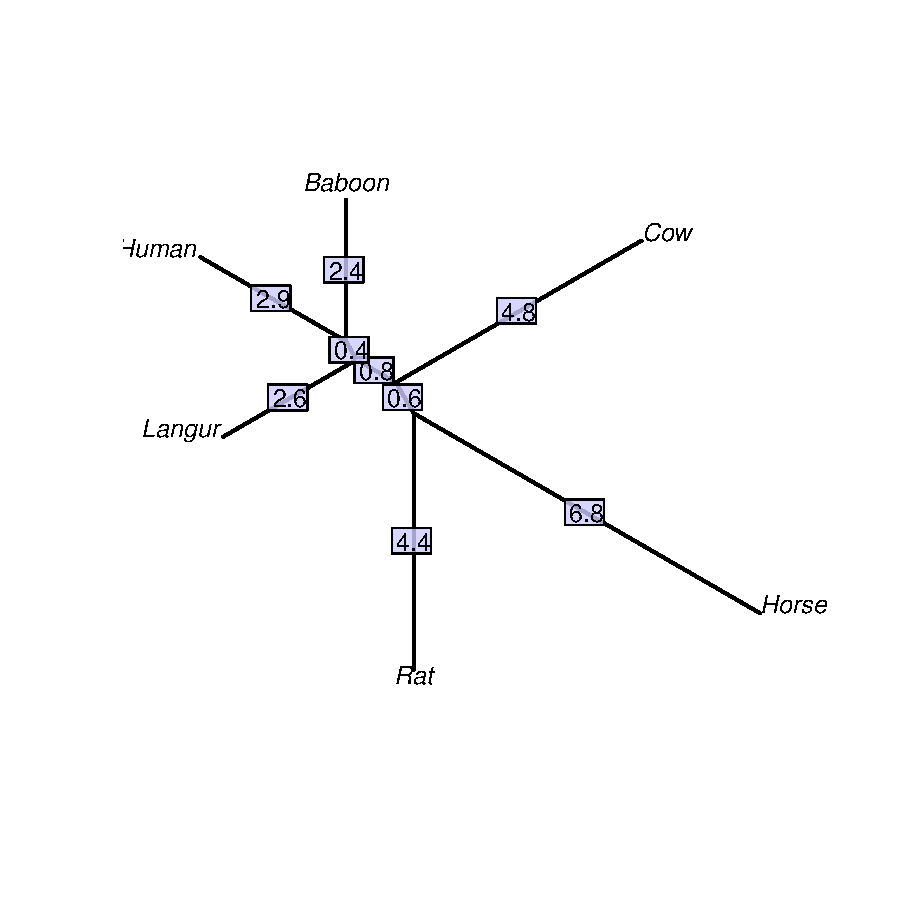
\includegraphics{figs/base-njAA}

The best possible planar representation of these Euclidean distances is achieved by Principal
Coordinate Analyses (PCoA), which in this case will give identical results to PCA of the original
(centred, non-scaled) data:
\begin{Schunk}
\begin{Sinput}
> pco1 <- dudi.pco(D, scannf = FALSE, nf = 2)
> scatter(pco1, posi = "bottomright")
> title("Principal Coordinate Analysis\n-based on proteic distances-")
\end{Sinput}
\end{Schunk}
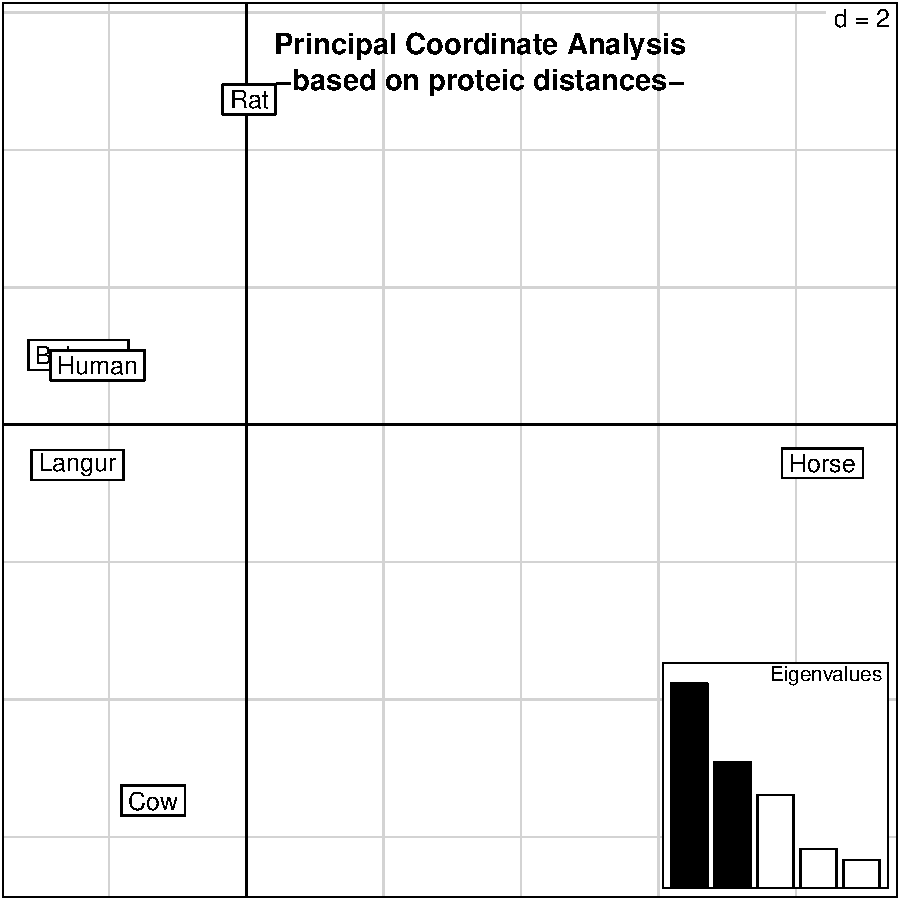
\includegraphics{figs/base-040}




%%%%%%%%%%%%%%%%%%%%%%%%%%%%%%%%%%%%%%%%%%%%%%%%%%
\subsection{Using genind/genpop constructors}
%%%%%%%%%%%%%%%%%%%%%%%%%%%%%%%%%%%%%%%%%%%%%%%%%%
Lastly, \texttt{genind} or \texttt{genpop} objects can be constructed from data matrices similar to the \texttt{\$tab} component (respectively, alleles frequencies and alleles counts).
This is achieved by the constructors \texttt{genind} (or \texttt{as.genind})  and \texttt{genpop}
(or \texttt{as.genpop}).
However, these low-level functions are first meant for internal use, and are called for instance by
functions such as \texttt{read.genetix}.
Consequently, there is much less control on the arguments and improper specification can lead to
creating improper \texttt{genind}/\texttt{genpop} objects without issuing a warning or an error, by
leading to meaningless subsequent analysis.

Therefore, one should use these functions with additional care as to how information is coded.
The table passed as argument to these constructors must have correct
names: unique rownames identifying genotypes/populations, and unique colnames
having the form '[marker].[allele]'.

Here is an example for \texttt{genpop} using a dataset from ade4:
\begin{Schunk}
\begin{Sinput}
> library(ade4)
> data(microsatt)
> microsatt$tab[10:15, 12:15]
\end{Sinput}
\begin{Soutput}
           INRA32.168 INRA32.170 INRA32.174 INRA32.176
Mtbeliard           0          0          0          1
NDama               0          0          0         12
Normand             1          0          0          2
Parthenais          8          5          0          3
Somba               0          0          0         20
Vosgienne           2          0          0          0
\end{Soutput}
\end{Schunk}
\texttt{microsatt\$tab} contains alleles counts per populations, and can therefore be used to make a \texttt{genpop} object.
Moreover, column names are set as required, and row names are unique.
It is therefore safe to convert these data into a \texttt{genpop} using the constructor:
\begin{Schunk}
\begin{Sinput}
> toto <- genpop(microsatt$tab)
> toto
\end{Sinput}
\begin{Soutput}
       #####################
       ### Genpop object ### 
       #####################
- Alleles counts for populations - 

S4 class:  genpop
@call: genpop(tab = microsatt$tab)

@tab:  18 x 112 matrix of alleles counts

@pop.names: vector of  18 population names
@loc.names: vector of  9 locus names
@loc.nall: number of alleles per locus
@loc.fac: locus factor for the  112 columns of @tab
@all.names: list of  9 components yielding allele names for each locus
@ploidy:  2
@type:  codom

@other: - empty -
\end{Soutput}
\begin{Sinput}
> summary(toto)
\end{Sinput}
\begin{Soutput}
 # Number of populations:  18 

 # Number of alleles per locus:  
L1 L2 L3 L4 L5 L6 L7 L8 L9 
 8 15 11 10 17 10 14 15 12 

 # Number of alleles per population:  
01 02 03 04 05 06 07 08 09 10 11 12 13 14 15 16 17 18 
39 69 51 59 52 41 34 48 46 47 43 56 57 52 49 64 56 67 

 # Percentage of missing data:  
[1] 0
\end{Soutput}
\end{Schunk}




%%%%%%%%%%%%%%%%%%%%%%%%%%%%%%%%%%%%%%%%%%%%%%%%%%
\subsection{Exporting data}
%%%%%%%%%%%%%%%%%%%%%%%%%%%%%%%%%%%%%%%%%%%%%%%%%%
Genotypes in \texttt{genind} format can be exported to the R packages
\emph{genetics} (using \texttt{genind2genotype}) and \emph{hierfstat} (using \texttt{genind2hierfstat}).
The package \emph{genetics} is now deprecated, but the implemented
class \texttt{genotype} is still used in various packages.
The package \emph{hierfstat} does not define a class, but requires
data to be formated in a particular way.
Here are examples of how to use these functions:
\begin{Schunk}
\begin{Sinput}
> obj <- genind2genotype(nancycats)
\end{Sinput}
\begin{Soutput}
NOTE: THIS PACKAGE IS NOW OBSOLETE.

  The R-Genetics project has developed an set of enhanced genetics
  packages to replace 'genetics'. Please visit the project homepage
  at http://rgenetics.org for informtion.
\end{Soutput}
\begin{Sinput}
> class(obj)
\end{Sinput}
\begin{Soutput}
[1] "data.frame"
\end{Soutput}
\begin{Sinput}
> obj[1:4, 1:5]
\end{Sinput}
\begin{Soutput}
         fca8   fca23   fca43   fca45   fca77
cat.1    <NA> 136/146 139/139 120/116 156/156
cat.2    <NA> 146/146 139/145 126/120 156/156
cat.3 135/143 136/146 141/141 116/116 156/152
cat.4 135/133 138/138 139/141 126/116 150/150
\end{Soutput}
\begin{Sinput}
> class(obj$fca8)
\end{Sinput}
\begin{Soutput}
[1] "genotype" "factor"  
\end{Soutput}
\end{Schunk}

\begin{Schunk}
\begin{Sinput}
> obj <- genind2hierfstat(nancycats)
> class(obj)
\end{Sinput}
\begin{Soutput}
[1] "data.frame"
\end{Soutput}
\begin{Sinput}
> obj[1:4, 1:5]
\end{Sinput}
\begin{Soutput}
      pop fca8 fca23 fca43 fca45
cat.1   1   NA   409   404   103
cat.2   1   NA   909   407   305
cat.3   1  913   409   505   101
cat.4   1  809   505   405   105
\end{Soutput}
\end{Schunk}

%% \noindent Now we can use the function \texttt{varcomp.glob} from
%% \emph{hierfstat} to compute 'variance' components:
%% <<echo=FALSE,eval=FALSE>>=
%% detach("package:ape")
%% @
%% <<>>=
%% varcomp.glob(obj$pop,obj[,-1])
%% @


A more generic way to export data is to produce a data.frame of genotypes
coded by character strings.
This is done by \texttt{genind2df}:
\begin{Schunk}
\begin{Sinput}
> obj <- genind2df(nancycats)
> obj[1:5, 1:5]
\end{Sinput}
\begin{Soutput}
      pop   fca8  fca23  fca43  fca45
cat.1   1   <NA> 136146 139139 116120
cat.2   1   <NA> 146146 139145 120126
cat.3   1 135143 136146 141141 116116
cat.4   1 133135 138138 139141 116126
cat.5   1 133135 140146 141145 126126
\end{Soutput}
\end{Schunk}

\noindent However, some software will require alleles to be
separated.
The argument \texttt{sep} allows one to specify any separator.
For instance:
\begin{Schunk}
\begin{Sinput}
> genind2df(nancycats, sep = "|")[1:5, 1:5]
\end{Sinput}
\begin{Soutput}
      pop    fca8   fca23   fca43   fca45
cat.1   1    <NA> 136|146 139|139 116|120
cat.2   1    <NA> 146|146 139|145 120|126
cat.3   1 135|143 136|146 141|141 116|116
cat.4   1 133|135 138|138 139|141 116|126
cat.5   1 133|135 140|146 141|145 126|126
\end{Soutput}
\end{Schunk}

Note that tabulations can be obtained as follows using '{$\backslash$}t' character.






\newpage
%%%%%%%%%%%%%%%%%%%%%%%%%%%%%%%%%%%%%%%%%%%%%%%%%%
%%%%%%%%%%%%%%%%%%%%%%%%%%%%%%%%%%%%%%%%%%%%%%%%%%
\section{Basics of data analysis}
%%%%%%%%%%%%%%%%%%%%%%%%%%%%%%%%%%%%%%%%%%%%%%%%%%
%%%%%%%%%%%%%%%%%%%%%%%%%%%%%%%%%%%%%%%%%%%%%%%%%%

%%%%%%%%%%%%%%%%%%%%%%%%%%%%%%%%%%%%%%%%%%%%%%%%%%
\subsection{Manipulating data}
%%%%%%%%%%%%%%%%%%%%%%%%%%%%%%%%%%%%%%%%%%%%%%%%%%
Data manipulation is meant to be easy in \textit{adegenet} (if it is
not, complain!).
First, as \texttt{genind} and \texttt{genpop} objects are basically formed
by a data matrix (the \texttt{@tab} slot), it is natural to subset these objects like it is done
with a matrix.
The \texttt{$[$} operator does this, forming a new object with the retained genotypes/populations and alleles:
\begin{Schunk}
\begin{Sinput}
> titi <- toto[1:3, ]
> toto$pop.names
\end{Sinput}
\begin{Soutput}
          01           02           03           04           05           06 
    "Baoule"     "Borgou"        "BPN"  "Charolais"   "Holstein"     "Jersey" 
          07           08           09           10           11           12 
 "Lagunaire"   "Limousin" "MaineAnjou"  "Mtbeliard"      "NDama"    "Normand" 
          13           14           15           16           17           18 
"Parthenais"      "Somba"  "Vosgienne"      "ZChoa"   "ZMbororo"      "Zpeul" 
\end{Soutput}
\begin{Sinput}
> titi
\end{Sinput}
\begin{Soutput}
       #####################
       ### Genpop object ### 
       #####################
- Alleles counts for populations - 

S4 class:  genpop
@call: .local(x = x, i = i, j = j, drop = drop)

@tab:  3 x 112 matrix of alleles counts

@pop.names: vector of  3 population names
@loc.names: vector of  9 locus names
@loc.nall: number of alleles per locus
@loc.fac: locus factor for the  112 columns of @tab
@all.names: list of  9 components yielding allele names for each locus
@ploidy:  2
@type:  codom

@other: a list containing: elements without names 
\end{Soutput}
\begin{Sinput}
> titi$pop.names
\end{Sinput}
\begin{Soutput}
       1        2        3 
"Baoule" "Borgou"    "BPN" 
\end{Soutput}
\end{Schunk}

\noindent The object \texttt{toto} has been subsetted, keeping only the
first three populations.
Of course, any subsetting available for a matrix can be used with \texttt{genind} and \texttt{genpop} objects.
For instance, we can subset \texttt{titi} to keep only the third marker:
\begin{Schunk}
\begin{Sinput}
> titi <- titi[, titi$loc.fac == "L3"]
> titi
\end{Sinput}
\begin{Soutput}
       #####################
       ### Genpop object ### 
       #####################
- Alleles counts for populations - 

S4 class:  genpop
@call: .local(x = x, i = i, j = j, drop = drop)

@tab:  3 x 11 matrix of alleles counts

@pop.names: vector of  3 population names
@loc.names: vector of  1 locus names
@loc.nall: number of alleles per locus
@loc.fac: locus factor for the  11 columns of @tab
@all.names: list of  1 components yielding allele names for each locus
@ploidy:  2
@type:  codom

@other: a list containing: elements without names 
\end{Soutput}
\end{Schunk}

\noindent Now, \texttt{titi} only contains the 11 alleles of the third
marker of \texttt{toto}.
\\

To simplify the task of separating data by marker, the function
\texttt{seploc} can be used.
It returns a list of objects (optionnaly, of data matrices), each
corresponding to a marker:
\begin{Schunk}
\begin{Sinput}
> sepCats <- seploc(nancycats)
> class(sepCats)
\end{Sinput}
\begin{Soutput}
[1] "list"
\end{Soutput}
\begin{Sinput}
> names(sepCats)
\end{Sinput}
\begin{Soutput}
[1] "fca8"  "fca23" "fca43" "fca45" "fca77" "fca78" "fca90" "fca96" "fca37"
\end{Soutput}
\begin{Sinput}
> sepCats$fca45
\end{Sinput}
\begin{Soutput}
   #####################
   ### Genind object ### 
   #####################
- genotypes of individuals - 

S4 class:  genind
@call: .local(x = x)

@tab:  237 x 9 matrix of genotypes

@ind.names: vector of  237 individual names
@loc.names: vector of  1 locus names
@loc.nall: number of alleles per locus
@loc.fac: locus factor for the  9 columns of @tab
@all.names: list of  1 components yielding allele names for each locus
@ploidy:  2
@type:  codom

Optionnal contents: 
@pop:  factor giving the population of each individual
@pop.names:  factor giving the population of each individual

@other: a list containing: xy 
\end{Soutput}
\end{Schunk}

\noindent The object \texttt{sepCats\$fca45} only contains data of the
marker fca45.
\\

Following the same idea, \texttt{seppop} allows one to separate genotypes
in a \texttt{genind} object by population.
For instance, we can separate genotype of cattles in the dataset \texttt{microbov}
by breed:
\begin{Schunk}
\begin{Sinput}
> data(microbov)
> obj <- seppop(microbov)
> class(obj)
\end{Sinput}
\begin{Soutput}
[1] "list"
\end{Soutput}
\begin{Sinput}
> names(obj)
\end{Sinput}
\begin{Soutput}
 [1] "Borgou"          "Zebu"            "Lagunaire"       "NDama"          
 [5] "Somba"           "Aubrac"          "Bazadais"        "BlondeAquitaine"
 [9] "BretPieNoire"    "Charolais"       "Gascon"          "Limousin"       
[13] "MaineAnjou"      "Montbeliard"     "Salers"         
\end{Soutput}
\begin{Sinput}
> obj$Borgou
\end{Sinput}
\begin{Soutput}
   #####################
   ### Genind object ### 
   #####################
- genotypes of individuals - 

S4 class:  genind
@call: .local(x = x, i = i, j = j, treatOther = ..1, quiet = ..2, drop = drop)

@tab:  50 x 373 matrix of genotypes

@ind.names: vector of  50 individual names
@loc.names: vector of  30 locus names
@loc.nall: number of alleles per locus
@loc.fac: locus factor for the  373 columns of @tab
@all.names: list of  30 components yielding allele names for each locus
@ploidy:  2
@type:  codom

Optionnal contents: 
@pop:  factor giving the population of each individual
@pop.names:  factor giving the population of each individual

@other: a list containing: coun  breed  spe 
\end{Soutput}
\end{Schunk}

\noindent The returned object \texttt{obj} is a list of \texttt{genind}
objects each containing genotypes of a given breed.

A last, rather vicious trick is to separate data by population and by marker.
This is easy using \texttt{lapply}; one can first separate population
then markers, or the contrary.
Here, we separate markers inside each breed in \texttt{obj}
\begin{Schunk}
\begin{Sinput}
> obj <- lapply(obj, seploc)
> names(obj)
\end{Sinput}
\begin{Soutput}
 [1] "Borgou"          "Zebu"            "Lagunaire"       "NDama"          
 [5] "Somba"           "Aubrac"          "Bazadais"        "BlondeAquitaine"
 [9] "BretPieNoire"    "Charolais"       "Gascon"          "Limousin"       
[13] "MaineAnjou"      "Montbeliard"     "Salers"         
\end{Soutput}
\begin{Sinput}
> class(obj$Borgou)
\end{Sinput}
\begin{Soutput}
[1] "list"
\end{Soutput}
\begin{Sinput}
> names(obj$Borgou)
\end{Sinput}
\begin{Soutput}
 [1] "INRA63"  "INRA5"   "ETH225"  "ILSTS5"  "HEL5"    "HEL1"    "INRA35" 
 [8] "ETH152"  "INRA23"  "ETH10"   "HEL9"    "CSSM66"  "INRA32"  "ETH3"   
[15] "BM2113"  "BM1824"  "HEL13"   "INRA37"  "BM1818"  "ILSTS6"  "MM12"   
[22] "CSRM60"  "ETH185"  "HAUT24"  "HAUT27"  "TGLA227" "TGLA126" "TGLA122"
[29] "TGLA53"  "SPS115" 
\end{Soutput}
\begin{Sinput}
> obj$Borgou$INRA63
\end{Sinput}
\begin{Soutput}
   #####################
   ### Genind object ### 
   #####################
- genotypes of individuals - 

S4 class:  genind
@call: .local(x = x)

@tab:  50 x 9 matrix of genotypes

@ind.names: vector of  50 individual names
@loc.names: vector of  1 locus names
@loc.nall: number of alleles per locus
@loc.fac: locus factor for the  9 columns of @tab
@all.names: list of  1 components yielding allele names for each locus
@ploidy:  2
@type:  codom

Optionnal contents: 
@pop:  factor giving the population of each individual
@pop.names:  factor giving the population of each individual

@other: a list containing: coun  breed  spe 
\end{Soutput}
\end{Schunk}

For instance, \texttt{obj\$Borgou\$INRA63} contains genotypes of the
breed Borgou for the marker INRA63.
\\

Lastly, one may want to pool genotypes in different datasets, but having
the same markers, into a single dataset.
This is more than just merging the \texttt{@tab} components of all
datasets, because alleles can differ (they almost always do) and
markers are not necessarily sorted the same way.
The function \texttt{repool} is designed to avoid these problems.
It can merge any \texttt{genind} provided as arguments as soon as the
same markers are used.
For instance, it can be used after a \texttt{seppop} to retain only some populations:
\begin{Schunk}
\begin{Sinput}
> obj <- seppop(microbov)
> names(obj)
\end{Sinput}
\begin{Soutput}
 [1] "Borgou"          "Zebu"            "Lagunaire"       "NDama"          
 [5] "Somba"           "Aubrac"          "Bazadais"        "BlondeAquitaine"
 [9] "BretPieNoire"    "Charolais"       "Gascon"          "Limousin"       
[13] "MaineAnjou"      "Montbeliard"     "Salers"         
\end{Soutput}
\begin{Sinput}
> newObj <- repool(obj$Borgou, obj$Charolais)
> newObj
\end{Sinput}
\begin{Soutput}
   #####################
   ### Genind object ### 
   #####################
- genotypes of individuals - 

S4 class:  genind
@call: repool(obj$Borgou, obj$Charolais)

@tab:  105 x 295 matrix of genotypes

@ind.names: vector of  105 individual names
@loc.names: vector of  30 locus names
@loc.nall: number of alleles per locus
@loc.fac: locus factor for the  295 columns of @tab
@all.names: list of  30 components yielding allele names for each locus
@ploidy:  2
@type:  codom

Optionnal contents: 
@pop:  factor giving the population of each individual
@pop.names:  factor giving the population of each individual

@other: - empty -
\end{Soutput}
\begin{Sinput}
> newObj$pop.names
\end{Sinput}
\begin{Soutput}
         P1          P2 
   "Borgou" "Charolais" 
\end{Soutput}
\end{Schunk}
Done !




%%%%%%%%%%%%%%%%%%%%%%%%%%%%%%%%%%%%%%%%%%%%%%%%%%
\subsection{Using summaries}
%%%%%%%%%%%%%%%%%%%%%%%%%%%%%%%%%%%%%%%%%%%%%%%%%%
Both \texttt{genind} and \texttt{genpop} objects have a summary providing basic information about data.
Informations are both printed and invisibly returned as a list.

\begin{Schunk}
\begin{Sinput}
> toto <- summary(nancycats)
\end{Sinput}
\begin{Soutput}
 # Total number of genotypes:  237 

 # Population sample sizes:  
 1  2  3  4  5  6  7  8  9 10 11 12 13 14 15 16 17 
10 22 12 23 15 11 14 10  9 11 20 14 13 17 11 12 13 

 # Number of alleles per locus:  
L1 L2 L3 L4 L5 L6 L7 L8 L9 
16 11 10  9 12  8 12 12 18 

 # Number of alleles per population:  
01 02 03 04 05 06 07 08 09 10 11 12 13 14 15 16 17 
36 53 50 67 48 56 42 54 43 46 70 52 44 61 42 40 35 

 # Percentage of missing data:  
[1] 2.344116

 # Observed heterozygosity:  
       L1        L2        L3        L4        L5        L6        L7        L8 
0.6682028 0.6666667 0.6793249 0.7083333 0.6329114 0.5654008 0.6497890 0.6184211 
       L9 
0.4514768 

 # Expected heterozygosity:  
       L1        L2        L3        L4        L5        L6        L7        L8 
0.8657224 0.7928751 0.7953319 0.7603095 0.8702576 0.6884669 0.8157881 0.7603493 
       L9 
0.6062686 
\end{Soutput}
\begin{Sinput}
> names(toto)
\end{Sinput}
\begin{Soutput}
[1] "N"        "pop.eff"  "loc.nall" "pop.nall" "NA.perc"  "Hobs"     "Hexp"    
\end{Soutput}
\begin{Sinput}
> par(mfrow = c(2, 2))
> plot(toto$pop.eff, toto$pop.nall, xlab = "Colonies sample size", 
+     ylab = "Number of alleles", main = "Alleles numbers and sample sizes", 
+     type = "n")
> text(toto$pop.eff, toto$pop.nall, lab = names(toto$pop.eff))
> barplot(toto$loc.nall, ylab = "Number of alleles", main = "Number of alleles per locus")
> barplot(toto$Hexp - toto$Hobs, main = "Heterozygosity: expected-observed", 
+     ylab = "Hexp - Hobs")
> barplot(toto$pop.eff, main = "Sample sizes per population", ylab = "Number of genotypes", 
+     las = 3)
\end{Sinput}
\end{Schunk}
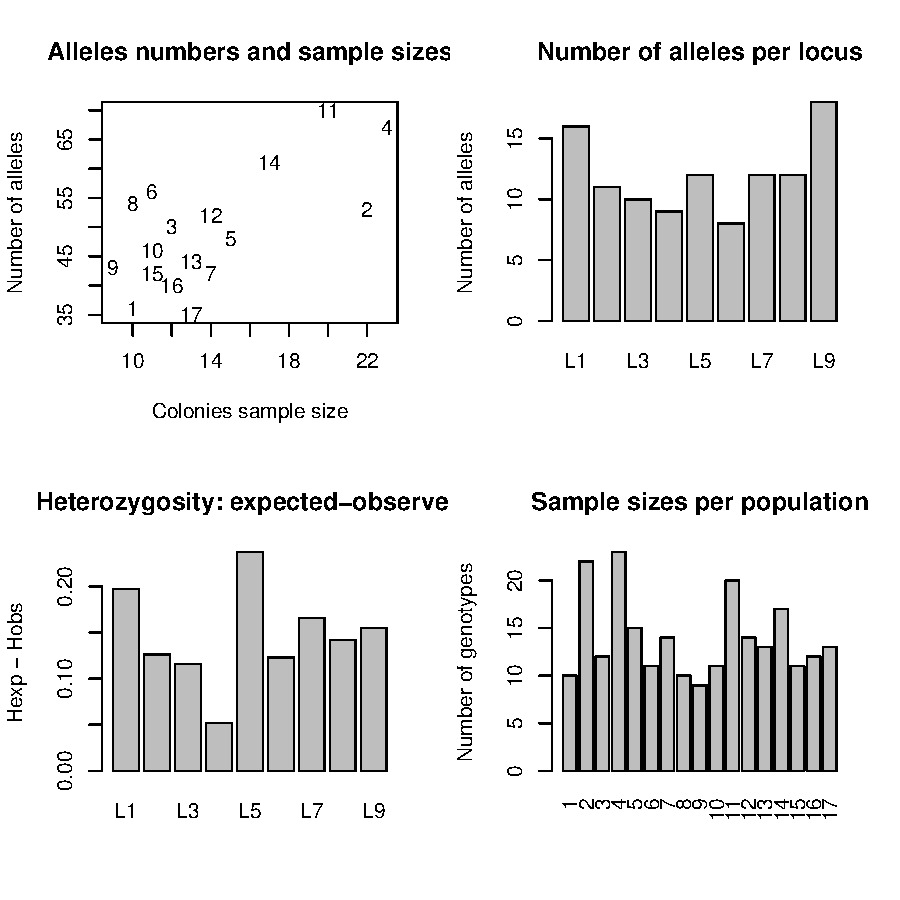
\includegraphics{figs/base-sumry}

Is mean observed H significantly lower than mean expected H ?

\begin{Schunk}
\begin{Sinput}
> bartlett.test(list(toto$Hexp, toto$Hobs))
\end{Sinput}
\begin{Soutput}
	Bartlett test of homogeneity of variances

data:  list(toto$Hexp, toto$Hobs) 
Bartlett's K-squared = 0.047, df = 1, p-value = 0.8284
\end{Soutput}
\begin{Sinput}
> t.test(toto$Hexp, toto$Hobs, pair = T, var.equal = TRUE, alter = "greater")
\end{Sinput}
\begin{Soutput}
	Paired t-test

data:  toto$Hexp and toto$Hobs 
t = 8.3294, df = 8, p-value = 1.631e-05
alternative hypothesis: true difference in means is greater than 0 
95 percent confidence interval:
 0.1134779       Inf 
sample estimates:
mean of the differences 
              0.1460936 
\end{Soutput}
\end{Schunk}
Yes, it is.





%%%%%%%%%%%%%%%%%%%%%%%%%%%%%%%%%%%%%%%%%%%%%%%%%%
\subsection{Testing for Hardy-Weinberg equilibrium}
%%%%%%%%%%%%%%%%%%%%%%%%%%%%%%%%%%%%%%%%%%%%%%%%%%
The Hardy-Weinberg equilibrium test is implemented for \texttt{genind} objects.
The function to use is \texttt{HWE.test.genind}, and requires the package \emph{genetics}.
Here we first produce a matrix of p-values (\texttt{res="matrix"}) using parametric test.
Monte Carlo procedure are more reliable but also more computer-intensive (use \texttt{permut=TRUE}).
\begin{Schunk}
\begin{Sinput}
> toto <- HWE.test.genind(nancycats, res = "matrix")
> dim(toto)
\end{Sinput}
\begin{Soutput}
[1] 17  9
\end{Soutput}
\end{Schunk}
One test is performed per locus and population, \textit{i.e.} 153 tests in this case.
Thus, the first question is: which tests are highly significant?
\begin{Schunk}
\begin{Sinput}
> colnames(toto)
\end{Sinput}
\begin{Soutput}
[1] "fca8"  "fca23" "fca43" "fca45" "fca77" "fca78" "fca90" "fca96" "fca37"
\end{Soutput}
\begin{Sinput}
> which(toto < 1e-04, TRUE)
\end{Sinput}
\begin{Soutput}
    row col
P14  14   2
P02   2   7
P02   2   8
P05   5   9
\end{Soutput}
\end{Schunk}
Here, only 4 tests indicate departure from HW.
Rows give populations, columns give markers.
Now complete tests are returned, but the significant ones are already known.
\begin{Schunk}
\begin{Sinput}
> toto <- HWE.test.genind(nancycats, res = "full")
> toto$fca23$P06
\end{Sinput}
\begin{Soutput}
	Pearson's Chi-squared test

data:  tab 
X-squared = 19.25, df = 10, p-value = 0.0372
\end{Soutput}
\begin{Sinput}
> toto$fca90$P10
\end{Sinput}
\begin{Soutput}
	Pearson's Chi-squared test

data:  tab 
X-squared = 19.25, df = 10, p-value = 0.0372
\end{Soutput}
\begin{Sinput}
> toto$fca96$P10
\end{Sinput}
\begin{Soutput}
	Pearson's Chi-squared test

data:  tab 
X-squared = 4.8889, df = 10, p-value = 0.8985
\end{Soutput}
\begin{Sinput}
> toto$fca37$P13
\end{Sinput}
\begin{Soutput}
	Pearson's Chi-squared test

data:  tab 
X-squared = 14.8281, df = 10, p-value = 0.1385
\end{Soutput}
\end{Schunk}





%%%%%%%%%%%%%%%%%%%%%%%%%%%%%%%%%%%%%%%%%%%%%%%%%%
\subsection{Measuring and testing population structure (a.k.a F statistics)}
%%%%%%%%%%%%%%%%%%%%%%%%%%%%%%%%%%%%%%%%%%%%%%%%%%
Population structure is traditionally measured and tested using F statistics, in particular Fst.
Since version 2.13.0 of R, the package \emph{hierfstat}, which implemented most F statistics and
related tests, has been removed from CRAN for maintenance issues.
As a consequence, \emph{adegenet} has lost a few functionalities, namely general F statistics
(function \texttt{fstat}) and a test of overall population structure (\texttt{gstat.randtest}).
\\


%% The first two are wrappers for functions implemented in the \emph{hierfstat} package; pairwise Fst
%% is implemented in \emph{adegenet}.

%% We illustrate their use using the dataset of microsatellite of cats from Nancy:
%% <<>>=
%% library(hierfstat)
%% data(nancycats)
%% fstat(nancycats)
%% @
%% This table provides the three F statistics $Fst$ (pop/total), $Fit$ (Ind/total), and $Fis$ (ind/pop).
%% These are overall measures which take into account all genotypes and all loci.

%% Is the structure between populations significant?
%% This question can be addressed using the G-statistic test \cite{tj511}; it is implemented for \texttt{genind} objects and produces a \texttt{randtest} object (package ade4).
%% <<fig=TRUE>>=
%% library(ade4)
%% toto <- gstat.randtest(nancycats,nsim=99)
%% toto
%% plot(toto)
%% @

%% \noindent Yes, it is (the observed value is indicated on the right, while histograms correspond to
%% the permuted values).
%% Note that \emph{hierfstat} allows for more ellaborated tests, in particular when different levels of
%% hierarchical clustering are available.
%% Such tests are better done directly in \emph{hierfstat}; for this, \texttt{genind} objects can be
%% converted to the adequat format using \texttt{genind2hierfstat}.
%% For instance:
%% <<>>=
%% toto <- genind2hierfstat(nancycats)
%% head(toto)
%% varcomp.glob(toto$pop,toto[,-1])
%% @
%% F statistics are provided in \$F; for instance, here, $F_{st}$ is $0.083$.


%% ~\\


However, it is still possible to compute pairwise $Fst$ using \textit{adegenet}.
Pairwise $Fst$ is frequently used as a measure of distance between populations.
The function \texttt{pairwise.fst} computes Nei's estimator \cite{tj814} of pairwise $Fst$, defined as:
$$
Fst(A,B) = \frac{H_t - (n_AH_s(A) + n_BH_s(B))/(n_A + n_B)}{Ht}
$$
where A and B refer to the two populations of sample size $n_A$ and $n_B$ and respective
expected heterozygosity $H_s(A)$ and $H_s(B)$, and $H_t$ is the expected heterozygosity in the whole dataset.
For a given locus, expected heterozygosity is computed as $1 - \sum p_i^2$, where $p_i$ is the
frequency of the $i$th allele, and the $\sum$ represents summation over all alleles.
For multilocus data, the heterozygosity is simply averaged over all loci.
These computations are achieved for all pairs of populations by the function \texttt{pairwise.fst}; we
illustrate this on a subset of individuals of \texttt{nancycats} (computations for the whole dataset
would take a few tens of seconds):
\begin{Schunk}
\begin{Sinput}
> data(nancycats)
> matFst <- pairwise.fst(nancycats[1:50, treatOther = FALSE])
> matFst
\end{Sinput}
\begin{Soutput}
           1          2          3
2 0.08018500                      
3 0.07140847 0.08200880           
4 0.08163151 0.06512457 0.04131227
\end{Soutput}
\end{Schunk}

The resulting matrix is Euclidean when there are no missing values:
\begin{Schunk}
\begin{Sinput}
> is.euclid(matFst)
\end{Sinput}
\begin{Soutput}
[1] TRUE
\end{Soutput}
\end{Schunk}

It can therefore be used in a Principal Coordinate Analysis (which requires Euclideanity), used to
build trees, etc.







%%%%%%%%%%%%%%%%%%%%%%%%%%%%%%%%%%%%%%%%%%%%%%%%%%
\subsection{Estimating inbreeding}
%%%%%%%%%%%%%%%%%%%%%%%%%%%%%%%%%%%%%%%%%%%%%%%%%%
Inbreeding refers to an excess of homozygosity in a given individual due to the mating of
genetically related parents.
This excess of homozygosity is due to the fact that there are non-negligible chances of inheriting
two identical alleles from a recent common ancestor.
Inbreeding can be associated to a loss of fitness leading to "\textit{inbreeding depression}".
Typically, loss of fitness is caused by recessive deleterious alleles which have usually low
frequency in the population, but for which inbred individuals are more likely to be homozygotes.
\\


The inbreeding coefficient $F$ is defined as the probability that at a given locus, two identical
alleles have been inherited from a common ancestor.
In the absence of inbreeding, the probability of being homozygote at one loci simply is (for diploid
individuals) simply $\sum_i p_i^2$ where $i$ indexes the alleles and $p_i$ is the frequency of
allele $i$.
This can be generalized incorporating $F$ as:
$$
p(\mbox{homozygote}) = F + (1-F) \sum_ip_i^2
$$
and even more generally, for any ploidy $\pi$:
$$
p(\mbox{homozygote}) = F + (1-F) \sum_ip_i^{\pi}
$$
This therefore allows for computing the likelihood of a given state (homozygote/heterozygote) in a
given genotype (log-likelihood are summed across loci for more than one marker).
\\

This estimation is achieved by \texttt{inbreeding}.
Depending on the value of the argument \texttt{res.type}, the function returns a sample from the
likelihood function (\texttt{res.type='sample'}) or the likelihood function itself, as a R function (\texttt{res.type='function'}).
While likelihood functions are quickly obtained and easy to display graphically, sampling from the
distributions is more computer intensive but may be useful if one wants to derive summary statistics of the distributions.
Here, we illustrate \texttt{inbreeding} using the \texttt{microbov} dataset, which contains cattle
breeds genotypes for 30 microsatellites; to focus on breed Salers only, we use \texttt{seppop}:
\begin{Schunk}
\begin{Sinput}
> data(microbov)
> sal <- seppop(microbov)$Salers
> sal
\end{Sinput}
\begin{Soutput}
   #####################
   ### Genind object ### 
   #####################
- genotypes of individuals - 

S4 class:  genind
@call: .local(x = x, i = i, j = j, treatOther = ..1, quiet = ..2, drop = drop)

@tab:  50 x 373 matrix of genotypes

@ind.names: vector of  50 individual names
@loc.names: vector of  30 locus names
@loc.nall: number of alleles per locus
@loc.fac: locus factor for the  373 columns of @tab
@all.names: list of  30 components yielding allele names for each locus
@ploidy:  2
@type:  codom

Optionnal contents: 
@pop:  factor giving the population of each individual
@pop.names:  factor giving the population of each individual

@other: a list containing: coun  breed  spe 
\end{Soutput}
\end{Schunk}
We first compute the mean inbreeding for each individual, and plot the resulting distribution:
\begin{Schunk}
\begin{Sinput}
> temp <- inbreeding(sal, N = 100)
> class(temp)
\end{Sinput}
\begin{Soutput}
[1] "list"
\end{Soutput}
\begin{Sinput}
> head(names(temp))
\end{Sinput}
\begin{Soutput}
[1] "FRBTSAL9087" "FRBTSAL9088" "FRBTSAL9089" "FRBTSAL9090" "FRBTSAL9091"
[6] "FRBTSAL9093"
\end{Soutput}
\end{Schunk}
\texttt{temp} is a list of values sampled from the likelihood distribution of each individual; means
values are obtained for all individuals using \texttt{sapply}:
\begin{Schunk}
\begin{Sinput}
> Fbar <- sapply(temp, mean)
\end{Sinput}
\end{Schunk}
\begin{Schunk}
\begin{Sinput}
> hist(Fbar, col = "firebrick", main = "Average inbreeding in Salers cattles")
\end{Sinput}
\end{Schunk}
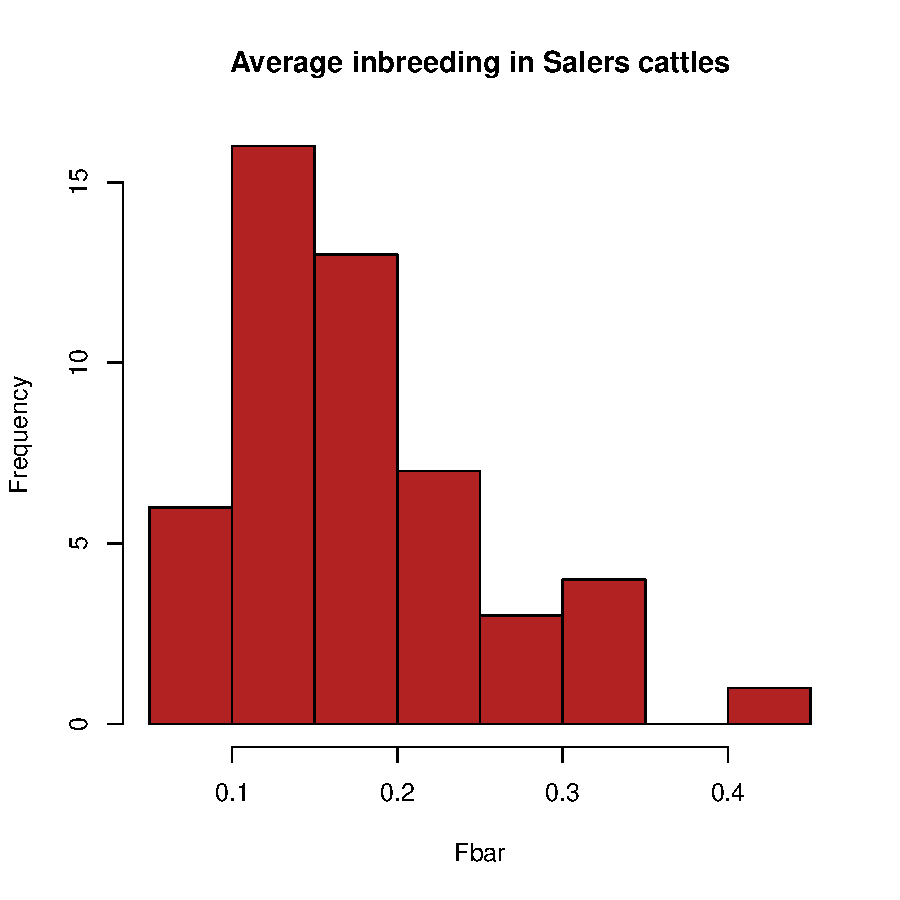
\includegraphics{figs/base-063}

\noindent We can see that some individuals (actually, a single one) have higher inbreeding (>0.4). We can recompute
inbreeding for this individual, asking for the likelihood function to be returned:
\begin{Schunk}
\begin{Sinput}
> which(Fbar > 0.4)
\end{Sinput}
\begin{Soutput}
FRBTSAL9266 
         37 
\end{Soutput}
\begin{Sinput}
> F <- inbreeding(sal, res.type = "function")[which(Fbar > 0.4)]
> F
\end{Sinput}
\begin{Soutput}
$FRBTSAL9266
function (F) 
{
    args <- lapply(as.list(match.call())[-1L], eval, parent.frame())
    names <- if (is.null(names(args))) 
        character(length(args))
    else names(args)
    dovec <- names %in% vectorize.args
    do.call("mapply", c(FUN = FUN, args[dovec], MoreArgs = list(args[!dovec]), 
        SIMPLIFY = SIMPLIFY, USE.NAMES = USE.NAMES))
}
<environment: 0x6e2d148>
\end{Soutput}
\end{Schunk}
The output object \texttt{F} can seem a bit cryptic: it is an function embedded within a hidden environment.
This does not matter, however, since it is easily represented:
\begin{Schunk}
\begin{Sinput}
> plot(F$FRBTSAL9266, main = paste("Inbreeding of individual", 
+     names(F)), xlab = "Inbreeding (F)", ylab = "Probability density")
\end{Sinput}
\end{Schunk}
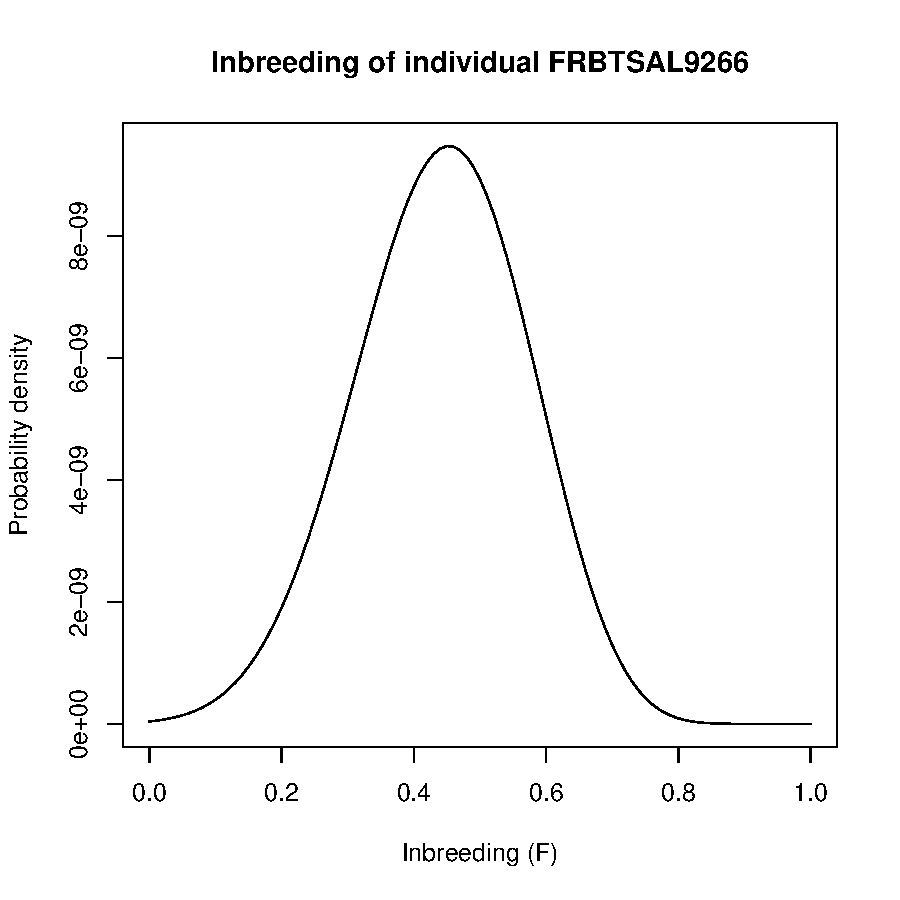
\includegraphics{figs/base-065}

\noindent Indeed, this individual shows subsequent inbreeding, with about 50\% chances of being
homozygote through inheritance from a common ancestor of its parents.






\newpage
%%%%%%%%%%%%%%%%%%%%%%%%%%%%%%%%%%%%%%%%%%%%%%%%%%
%%%%%%%%%%%%%%%%%%%%%%%%%%%%%%%%%%%%%%%%%%%%%%%%%%
\section{Multivariate analysis}
%%%%%%%%%%%%%%%%%%%%%%%%%%%%%%%%%%%%%%%%%%%%%%%%%%
%%%%%%%%%%%%%%%%%%%%%%%%%%%%%%%%%%%%%%%%%%%%%%%%%%

%%%%%%%%%%%%%%%%%%%%%%%%%%%%%%%%%%%%%%%%%%%%%%%%%%
\subsection{General overview}
%%%%%%%%%%%%%%%%%%%%%%%%%%%%%%%%%%%%%%%%%%%%%%%%%%

Multivariate analysis consists in summarising a strongly multivariate information into a few
synthetic variables.
In genetics, such approaches are useful to get a simplified picture of the genetic diversity
obersved amongst individuals or populations.
A review of multivariate analysis in population genetics can be found in \cite{tjart10}.
Here, we aim at providing an overview of some applications using methods implemented in \textit{ade4}
and \textit{adegenet}.
\\


Useful functions include:
\begin{itemize}
  \item \texttt{scaleGen} (\textit{adegenet}): centre/scale allele frequencies and replaces missing
    data; useful, among other things, before running a principal component analysis (PCA).
  \item \texttt{dudi.pca} (\textit{ade4}): implements PCA; can be used on transformed allele
    frequencies of individuals or populations.
  \item \texttt{dudi.ca} (\textit{ade4}): implements Correspondance Analysis (CA); can be used on raw
    allele counts of populations (\texttt{@tab} slot in \texttt{genpop} objects).
  \item \texttt{dist.genpop} (\textit{adegenet}): implements 5 pairwise genetic distances between populations
  \item \texttt{pairwise.fst} (\textit{adegenet}): implements pairwise $F_{ST}$, which is also a
    Euclidean distance between populations.
  \item \texttt{dist} (\textit{stats}): computes pairwise distances between multivariate
    observations; can be used on raw or transformed allele frequencies.
  \item \texttt{dudi.pco} (\textit{ade4}): implements Principal Coordinates Analysis (PCoA); this
    methods finds synthetic variables which summarize a Euclidean distance matrix as best as
    possible; can be used on outputs of \texttt{dist}, \texttt{dist.genpop}, and \texttt{pairwise.fst}.
  \item \texttt{is.euclid} (\textit{ade4}): tests whether a distance matrix is Euclidean, which is a
    pre-requisite of PCoA.
  \item \texttt{cailliez} (\textit{ade4}): renders a non-Euclidean distance matrix Euclidean by
    adding a constant to all entries.
  \item \texttt{dapc} (\textit{adegenet}): implements the Discriminant Analysis of Principal
    Components (DAPC \cite{tjart19}), a new standard method for the analysis of population genetic structures; see
    dedicated vignette (\textit{adegenet-dapc}).
  \item \texttt{sPCA} (\textit{adegenet}): implements the spatial Principal Component Analysis
    (sPCA \cite{tjart04}), a method for the analysis of spatial genetic structures; see dedicated vignette (\textit{adegenet-dapc}).
  \item \texttt{glPca} (\textit{adegenet}): implements PCA for genome-wide SNP data stored as
    \texttt{genlight} objects; see dedicated vignette (\textit{adegenet-genomics}).
    %% \item \texttt{} (\textit{}):
\end{itemize}

Besides the procedures themselves, graphic functions are also often of the utmost importance; these include:
\begin{itemize}
  \item \texttt{scatter} (\textit{ade4,adegenet}): generic function to display multivariate
    analyses; in practice, the only useful application for genetic data is the one implemented in
    \texttt{adegenet} for DAPC results.
  \item \texttt{s.label} (\textit{ade4}): function used for basic display of principal components.
  \item \texttt{loadingplot} (\textit{adegenet}): function used to display the loadings (i.e.,
    contribution to a given structure) of alleles for a given principal component; annotates and returns the most
    contributing alleles.
  \item \texttt{s.class} (\textit{ade4}): displays two quantitative variables with known groups of
    observations, using inertia ellipses for the groups; useful to represent principal components
    when groups are known.
  \item \texttt{s.chull} (\textit{ade4}): same as \texttt{s.class}, except convex polygons are used
    rather than ellipses.
  \item \texttt{s.value} (\textit{ade4}): graphical display of a quantitative variable distributed
    over a two-dimensional space; useful to map principal components or allele frequencies over a
    geographic area.
  \item \texttt{colorplot} (\textit{adegenet}): graphical display of 1 to 3 quantitative variables distributed
    over a two-dimensional space; useful for combined representations of principal components over a geographic area.
    Can also be used to produce color versions of traditional scatterplots.
  \item \texttt{transp} (\textit{adegenet}): auxiliary function making colors transparent.
  \item \texttt{num2col} (\textit{adegenet}): auxiliary function transforming a quantitative
    variable into colors using a given palette.
  \item \texttt{assignplot} (\textit{adegenet}): specific plot of group membership probabilities for
    DAPC; see dedicated vignette (\textit{adegenet-dapc}).
  \item \texttt{compoplot} (\textit{adegenet}): specific 'STRUCTURE-like' plot of group membership probabilities for
    DAPC; see dedicated vignette (\textit{adegenet-dapc}).
  \item \texttt{add.scatter} (\textit{ade4}): add inset plots to an existing figure.
  %% \item \texttt{} (\textit{}): .
  %% \item \texttt{} (\textit{}): .
  %% \item \texttt{} (\textit{}): .
  %% \item \texttt{} (\textit{}): .
  %% \item \texttt{} (\textit{}): .
\end{itemize}

\noindent In the sections below, we briefly illustrate how these tools can be combined to extract information from
genetic data.




%%%%%%%%%%%%%%%%%%%%%%%%%%%%%%%%%%%%%%%%%%%%%%%%%%
\subsection{Performing a Principal Component Analysis on \texttt{genind} objects}
%%%%%%%%%%%%%%%%%%%%%%%%%%%%%%%%%%%%%%%%%%%%%%%%%%
The tables contained in \texttt{genind} objects can be submitted to a Principal Component Analysis (PCA) to seek a typology of individuals.
Such analysis is straightforward using \textit{adegenet} to prepare data and \textit{ade4} for the analysis \textit{per se}.
One has first to replace missing data.
Putting each missing observation at the mean of the concerned allele frequency seems the best choice (NA will be stuck at the origin).
\begin{Schunk}
\begin{Sinput}
> data(microbov)
> any(is.na(microbov$tab))
\end{Sinput}
\begin{Soutput}
[1] TRUE
\end{Soutput}
\begin{Sinput}
> sum(is.na(microbov$tab))
\end{Sinput}
\begin{Soutput}
[1] 6325
\end{Soutput}
\end{Schunk}
There are 6325 missing data.
Assuming that these are evenly distributed (for illustration purpose
only!), we replace them using \texttt{na.replace}.
As we intend to use a PCA, the appropriate replacement method is to
put each NA at the mean of the corresponding allele (argument 'method'
set to 'mean').
\begin{Schunk}
\begin{Sinput}
> obj <- na.replace(microbov, method = "mean")
\end{Sinput}
\begin{Soutput}
 Replaced 6325 missing values 
\end{Soutput}
\end{Schunk}

\noindent Note that alternatively, we could have used \texttt{scaleGen} to obtain centred/scaled
allele frequencies and replace NA.
\\

The analysis can now be performed.
Data are centred but not scaled as 'units' are the same.
Note: in practice, retained axes can be chosen interactively by removing the arguments \texttt{scannf=FALSE,nf=3}.
\begin{Schunk}
\begin{Sinput}
> pca1 <- dudi.pca(obj$tab, cent = TRUE, scale = FALSE, scannf = FALSE, 
+     nf = 3)
> barplot(pca1$eig[1:50], main = "PCA eigenvalues", col = heat.colors(50))
\end{Sinput}
\end{Schunk}
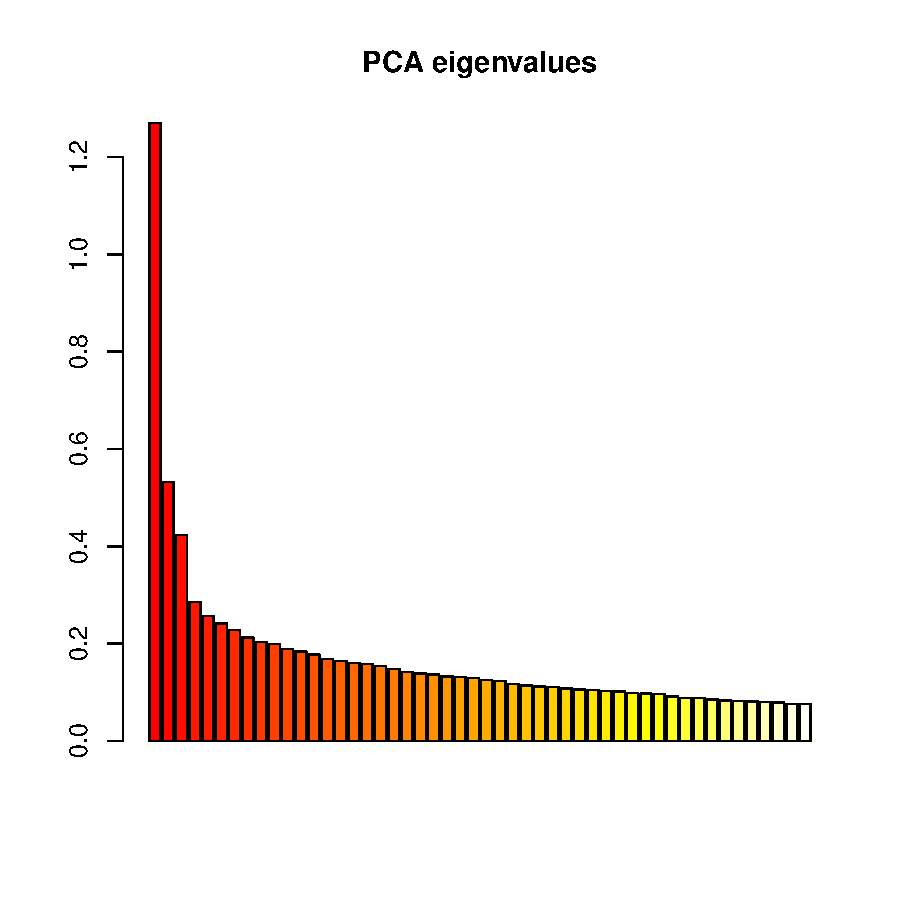
\includegraphics{figs/base-068}
\begin{Schunk}
\begin{Sinput}
> pca1
\end{Sinput}
\begin{Soutput}
Duality diagramm
class: pca dudi
$call: dudi.pca(df = obj$tab, center = TRUE, scale = FALSE, scannf = FALSE, 
    nf = 3)

$nf: 3 axis-components saved
$rank: 341
eigen values: 1.27 0.5317 0.423 0.2853 0.2565 ...
  vector length mode    content       
1 $cw    373    numeric column weights
2 $lw    704    numeric row weights   
3 $eig   341    numeric eigen values  

  data.frame nrow ncol content             
1 $tab       704  373  modified array      
2 $li        704  3    row coordinates     
3 $l1        704  3    row normed scores   
4 $co        373  3    column coordinates  
5 $c1        373  3    column normed scores
other elements: cent norm 
\end{Soutput}
\end{Schunk}
The output object \texttt{pca1} is a list containing various information; of particular interest are:
\begin{itemize}
\item \texttt{\$eig}: the eigenvalues of the analysis, indicating the amount of variance represented
  by each principal component (PC).
\item \texttt{\$li}: the principal components of the analysis; these are the synthetic variables
  summarizing the genetic diversity, usually visualized using scatterplots.
\item \texttt{\$c1}: the allele loadings, used to compute linear combinations forming the PCs;
  squared, they represent the contribution to each PCs.
\end{itemize}

The basic scatterplot for this analysis can be obtained by:
\begin{Schunk}
\begin{Sinput}
> s.label(pca1$li)
> title("PCA of microbov dataset\naxes 1-2")
> add.scatter.eig(pca1$eig[1:20], 3, 1, 2)
\end{Sinput}
\end{Schunk}
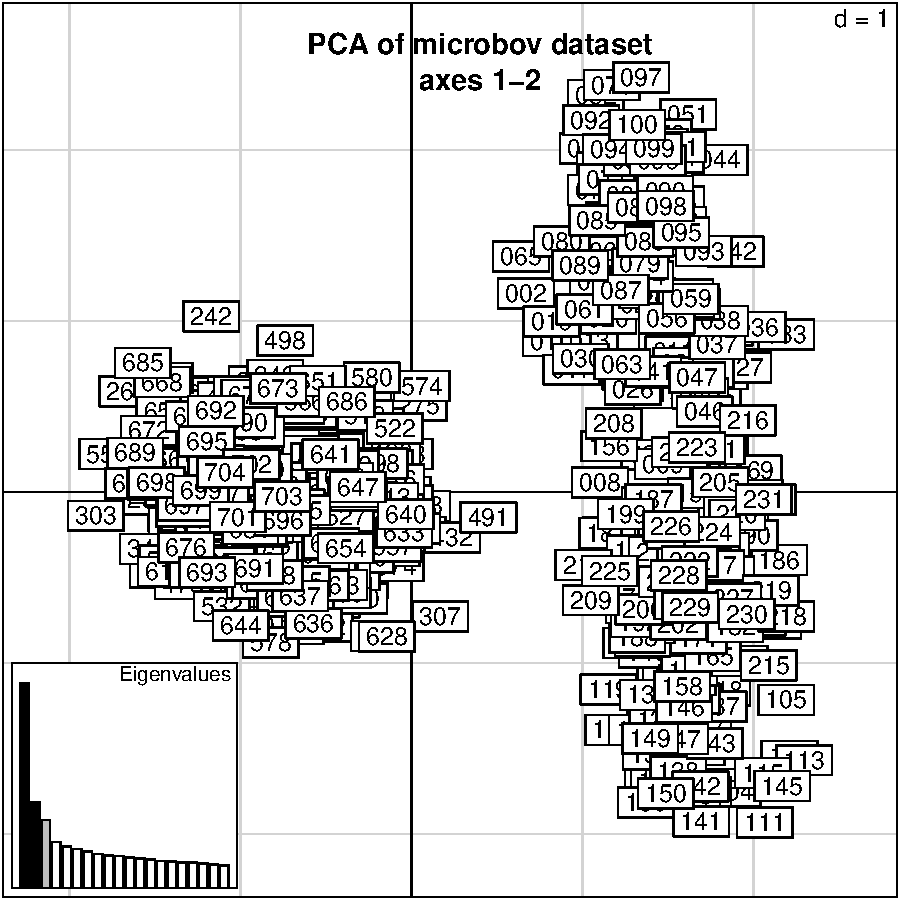
\includegraphics{figs/base-070}

\noindent However, this figure can largely be improved.
First, we can use \texttt{s.class} to represent both the genotypes and inertia ellipses for populations.
\begin{Schunk}
\begin{Sinput}
> s.class(pca1$li, pop(obj), lab = obj$pop.names)
> title("PCA of microbov dataset\naxes 1-2")
> add.scatter.eig(pca1$eig[1:20], 3, 1, 2)
\end{Sinput}
\end{Schunk}
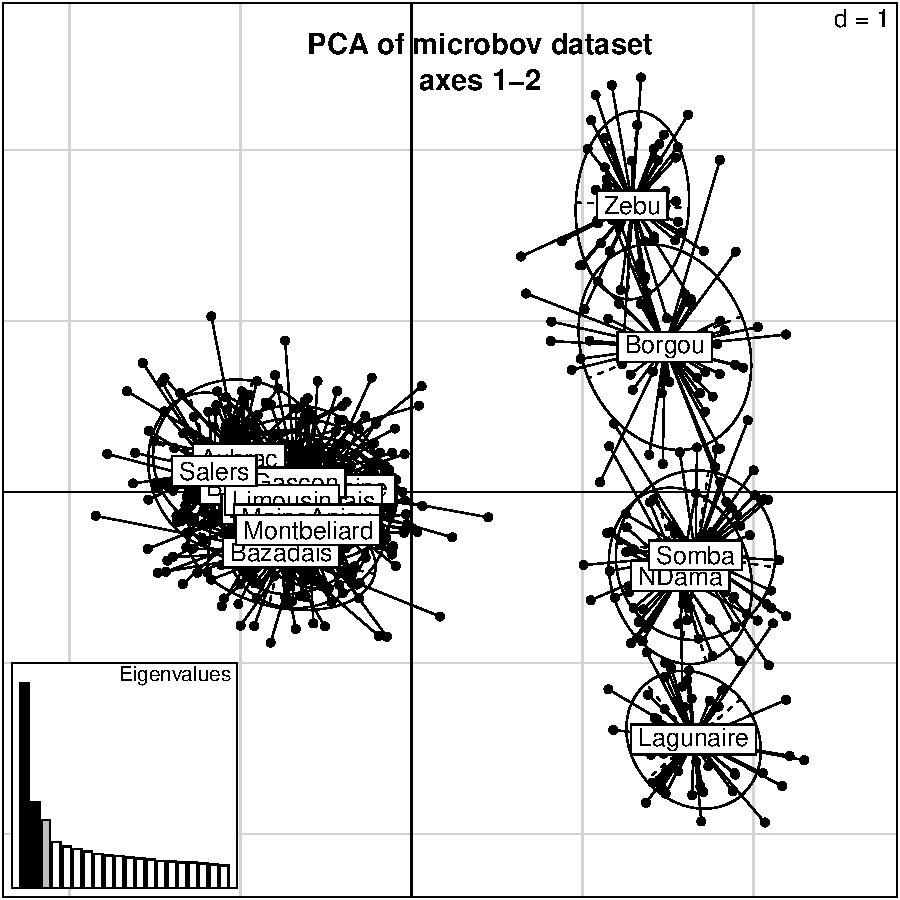
\includegraphics{figs/base-071}

\noindent This plane shows that the main structuring is between African an French breeds, the second structure reflecting genetic diversity among African breeds.
The third axis reflects the diversity among French breeds:
\begin{Schunk}
\begin{Sinput}
> s.class(pca1$li, pop(obj), xax = 1, yax = 3, lab = obj$pop.names, 
+     sub = "PCA 1-3", csub = 2)
> title("PCA of microbov dataset\naxes 1-3")
> add.scatter.eig(pca1$eig[1:20], nf = 3, xax = 1, yax = 3)
\end{Sinput}
\end{Schunk}
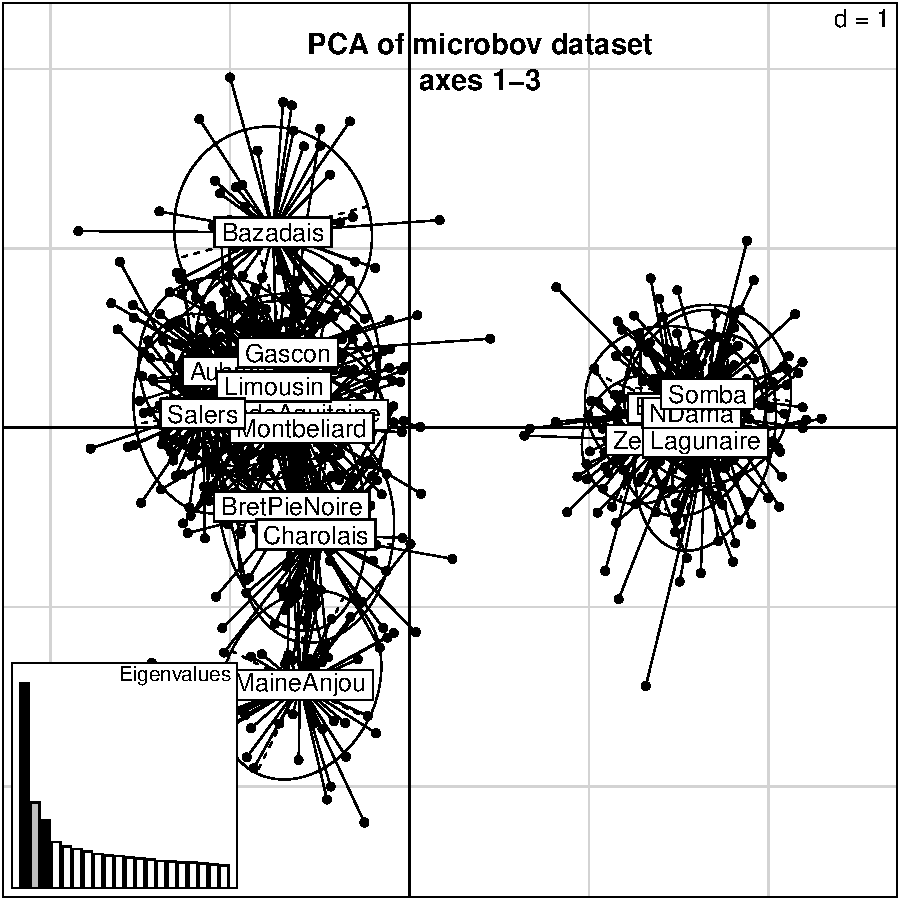
\includegraphics{figs/base-072}

\noindent Overall, all breeds seem well differentiated.
~\\

However, we can yet improve these scatterplots, which are fortunately easy to customize.
For instance, we can remove the grid, choose different colors for the groups, use larger dots and transparency to
better assess the density of points, and remove internal segments of the ellipses:
\begin{Schunk}
\begin{Sinput}
> col <- rainbow(length(levels(pop(obj))))
> s.class(pca1$li, pop(obj), xax = 1, yax = 3, col = transp(col, 
+     0.6), axesell = FALSE, cstar = 0, cpoint = 3, grid = FALSE)
\end{Sinput}
\end{Schunk}
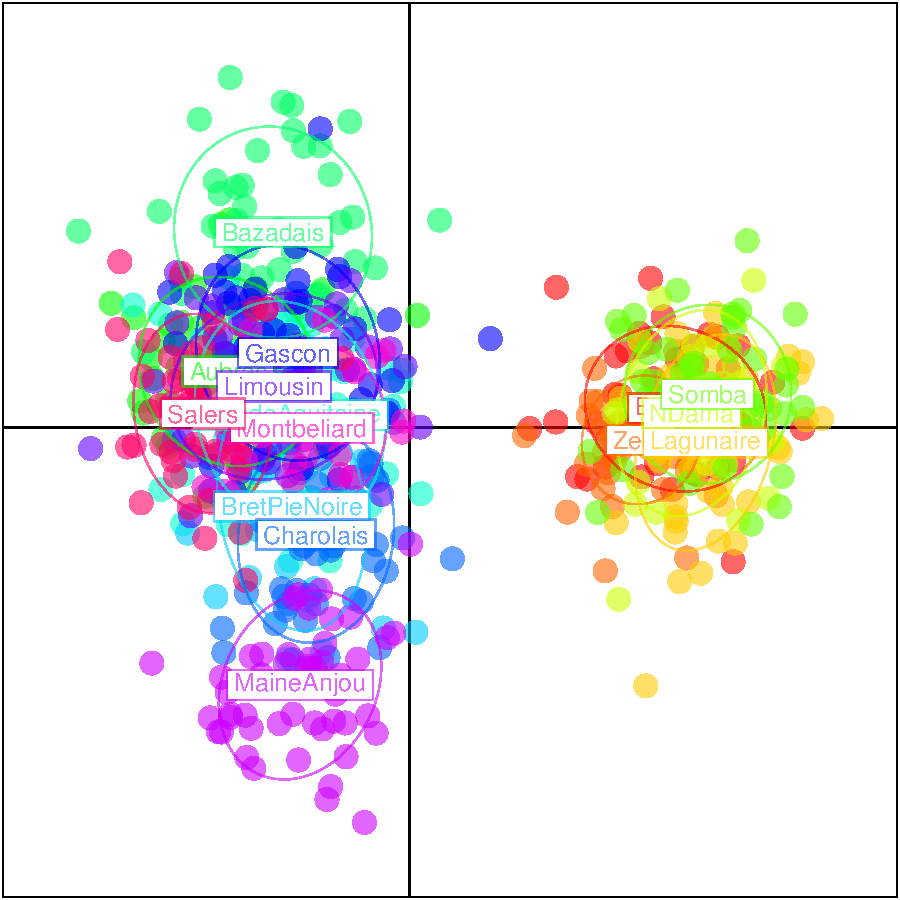
\includegraphics{figs/base-073}
~\\


Let us now assume that we ignore the group memberships.
We can still use color in an informative way.
For instance, we can recode the principal components represented in the scatterplot on the RGB
scale:
\begin{Schunk}
\begin{Sinput}
> colorplot(pca1$li, pca1$li, transp = TRUE, cex = 3, xlab = "PC 1", 
+     ylab = "PC 2")
> title("PCA of microbov dataset\naxes 1-2")
> abline(v = 0, h = 0, col = "grey", lty = 2)
\end{Sinput}
\end{Schunk}
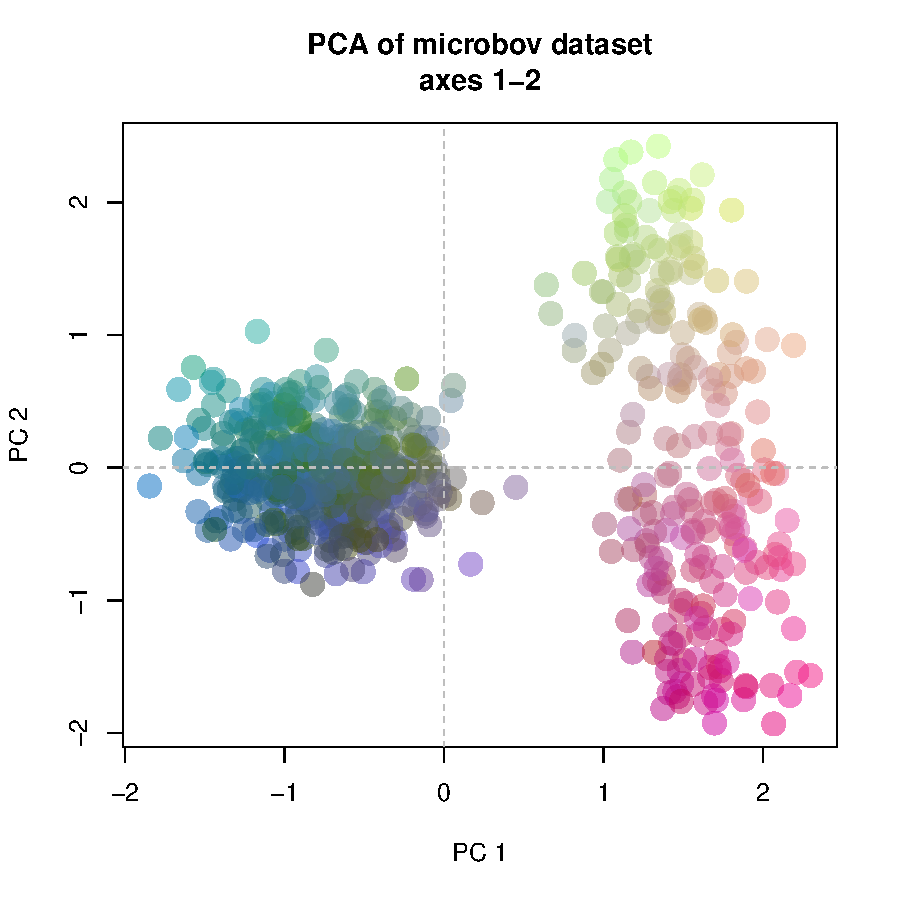
\includegraphics{figs/base-074}

\noindent Colors are based on the first three PCs of the PCA, recoded respectively on the red, green, and blue channel.
In this figure, the genetic diversity is represented in two redundant ways: by the distances
(further away = more genetically different), and by the colors (more different colors = more
genetically different).
\\

We can represent the diversity on the third axis similarly:
\begin{Schunk}
\begin{Sinput}
> colorplot(pca1$li[c(1, 3)], pca1$li, transp = TRUE, cex = 3, 
+     xlab = "PC 1", ylab = "PC 3")
> title("PCA of microbov dataset\naxes 1-3")
> abline(v = 0, h = 0, col = "grey", lty = 2)
\end{Sinput}
\end{Schunk}
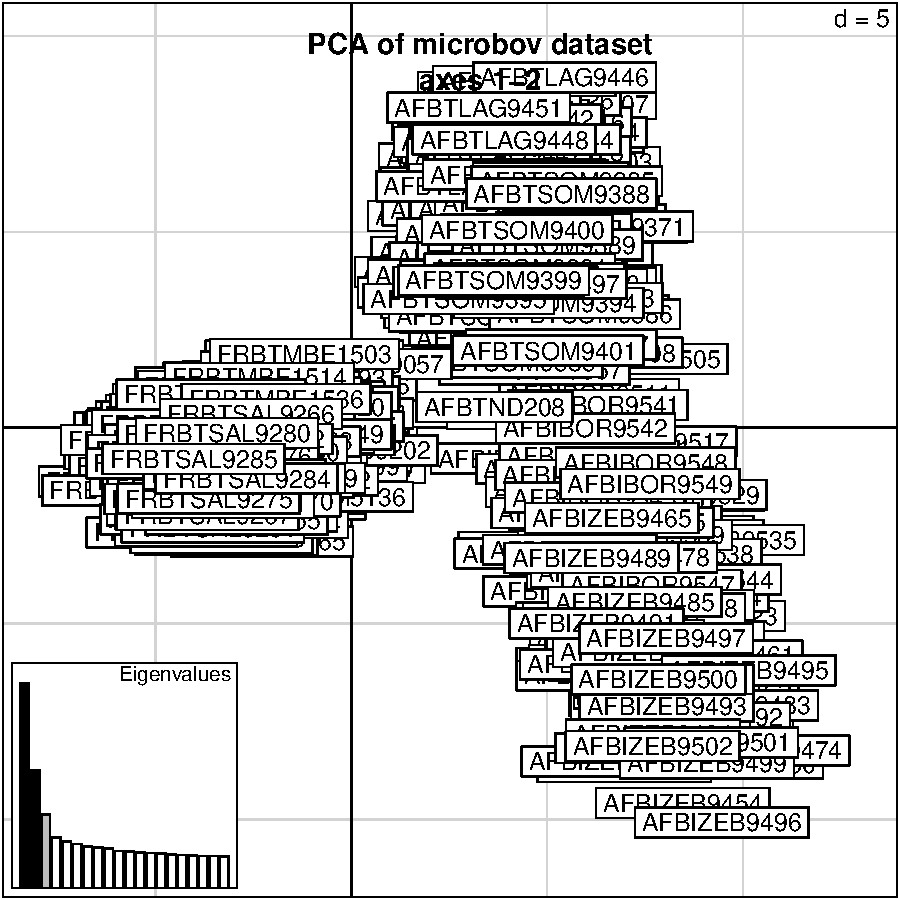
\includegraphics{figs/base-075}





%%%%%%%%%%%%%%%%%%%%%%%%%%%%%%%%%%%%%%%%%%%%%%%%%%
\subsection{Performing a Correspondance Analysis on \texttt{genpop} objects}
%%%%%%%%%%%%%%%%%%%%%%%%%%%%%%%%%%%%%%%%%%%%%%%%%%
Being contingency tables, the \texttt{@tab} slot in \texttt{genpop} objects can be submitted to a Correspondance Analysis (CA) to seek a typology of populations.
The approach is very similar to the previous one for PCA.
Missing data are first replaced during convertion from \texttt{genind},
but one could create a \texttt{genpop} with NAs and then use
\texttt{na.replace} to get rid of missing observations.
\begin{Schunk}
\begin{Sinput}
> data(microbov)
> obj <- genind2genpop(microbov, missing = "chi2")
\end{Sinput}
\begin{Soutput}
 Converting data from a genind to a genpop object... 

 Replaced 0 missing values 

...done.
\end{Soutput}
\begin{Sinput}
> ca1 <- dudi.coa(as.data.frame(obj$tab), scannf = FALSE, nf = 3)
> barplot(ca1$eig, main = "Correspondance Analysis eigenvalues", 
+     col = heat.colors(length(ca1$eig)))
\end{Sinput}
\end{Schunk}
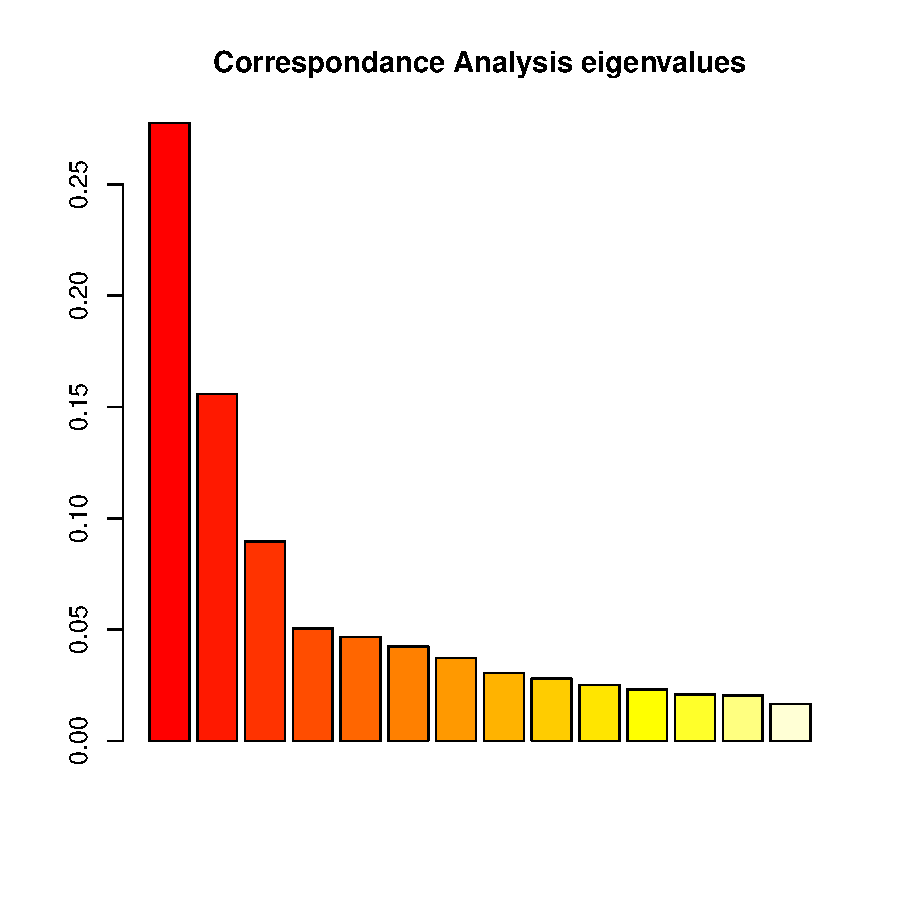
\includegraphics{figs/base-caexpl}

Now we display the resulting typology using a basic scatterplot:
\begin{Schunk}
\begin{Sinput}
> s.label(ca1$li, lab = obj$pop.names, sub = "CA 1-2", csub = 2)
> add.scatter.eig(ca1$eig, nf = 3, xax = 1, yax = 2, posi = "bottomright")
\end{Sinput}
\end{Schunk}
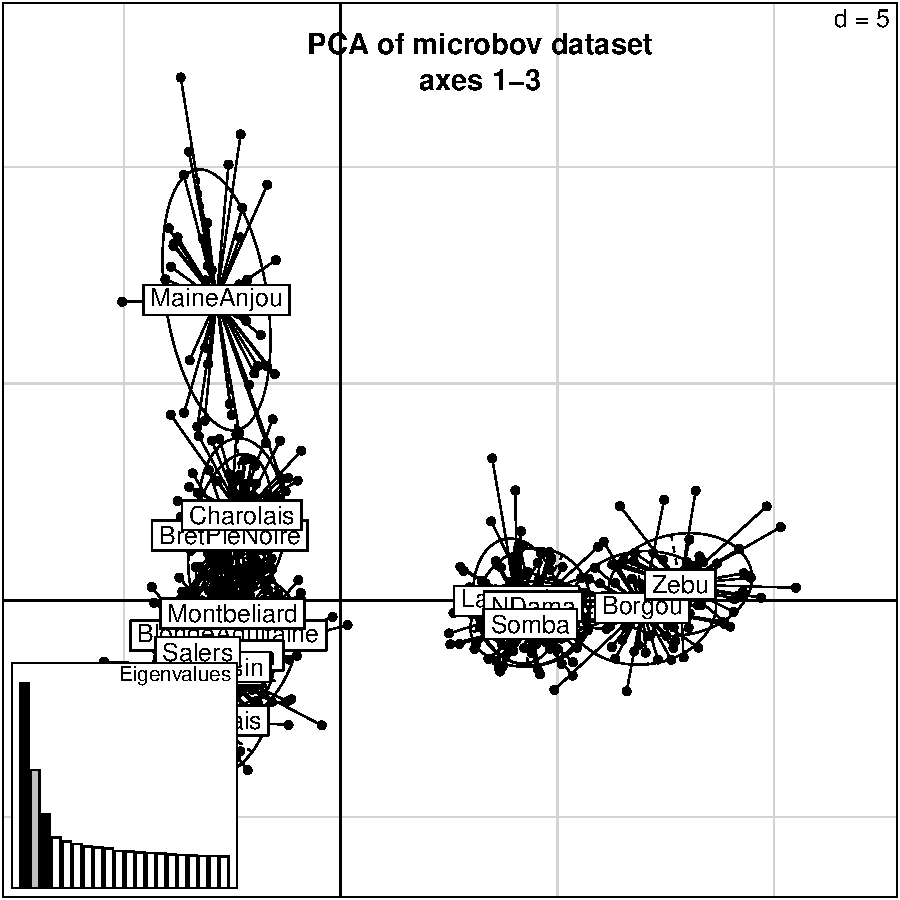
\includegraphics{figs/base-077}

\begin{Schunk}
\begin{Sinput}
> s.label(ca1$li, xax = 1, yax = 3, lab = obj$pop.names, sub = "CA 1-3", 
+     csub = 2)
> add.scatter.eig(ca1$eig, nf = 3, xax = 2, yax = 3, posi = "topleft")
\end{Sinput}
\end{Schunk}
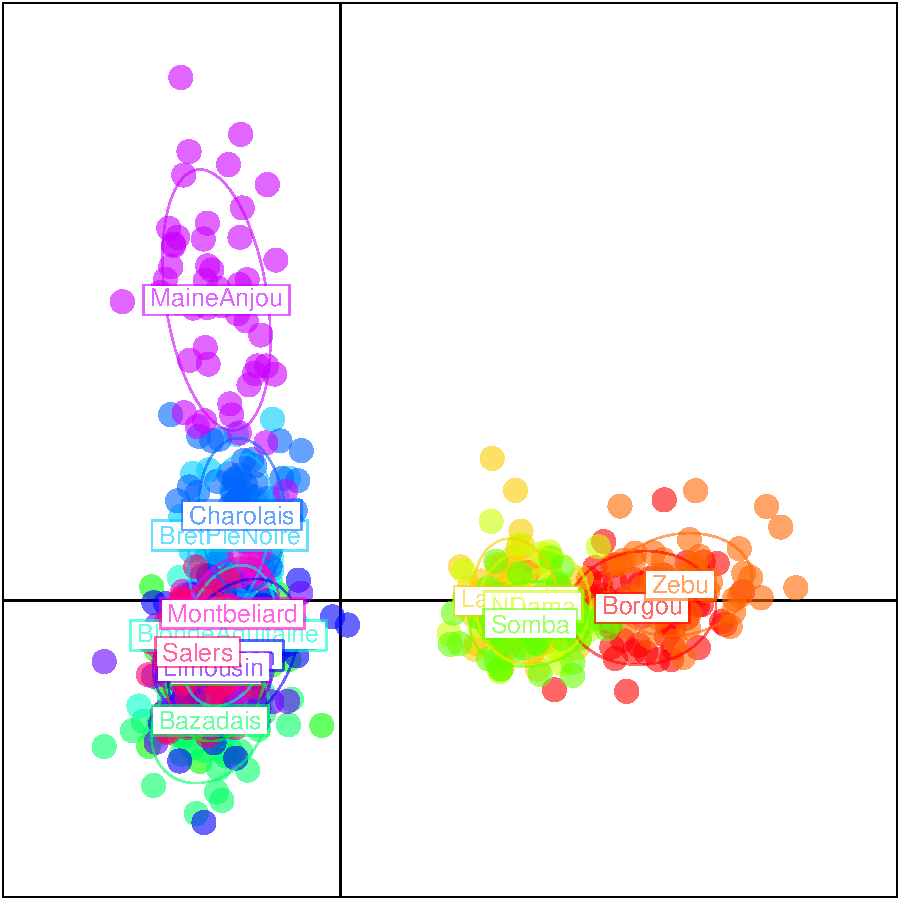
\includegraphics{figs/base-078}

\noindent As in the PCA above, axes are to be interpreted separately in terms of continental differentiation, and between-breeds diversity.
Importantly, as in any analysis carried out at a population level, all information about the
diversity within populations is lost in this analysis.
See the vignette on DAPC for an individual-based approach which is nontheless optimal in terms of
group separation (\textit{adegenet-dapc}).





%% %%%%%%%%%%%%%%%%%%%%%%%%%%%%%%%%%%%%%%%%%%%%%%%%%%
%% \subsection{Analyzing a single locus}
%% %%%%%%%%%%%%%%%%%%%%%%%%%%%%%%%%%%%%%%%%%%%%%%%%%%
%% Here the emphasis is put on analyzing a single locus using different methods.
%% Any marker can be isolated using the \texttt{seploc} instruction.
%% <<pca>>=
%% data(nancycats)
%% toto <- seploc(nancycats,truenames=TRUE, res.type="matrix")
%% X <- toto$fca90
%% @
%% \texttt{fca90.ind} is a matrix containing only genotypes for the marker fca90.
%% It can be analyzed, for instance, using an inter-class PCA.
%% This analyzis provides a typology of individuals having maximal inter-colonies variance.
%% <<fig=T,png=F,pdf=T>>=
%% library(ade4)

%% pcaX <- dudi.pca(X,cent=T,scale=F,scannf=FALSE)
%% pcabetX <- between(pcaX,nancycats$pop,scannf=FALSE)
%% s.arrow(pcabetX$c1,xlim=c(-.9,.9))
%% s.class(pcabetX$ls,nancycats$pop,cell=0,cstar=0,add.p=T)
%% sunflowerplot(X %*% as.matrix(pcabetX$c1),add=T)
%% add.scatter.eig(pcabetX$eig,xax=1,yax=2,posi="bottomright")
%% @
%% Here the differences between individuals are mainly expressed by three alleles: 199, 197 and 193.
%% However, there is no clear structuration to be seen at an individual level.
%% Is $F_{st}$ significant taking only this marker into account?
%% We perform the G-statistic test and enventually compute the corresponding F statistics.
%% Note that we use the constructor \texttt{genind} to generate an object
%% of this class from \texttt{X}:
%% <<>>=
%% fca90.ind <- genind(X,pop=nancycats$pop)
%% gstat.randtest(fca90.ind,nsim=999)
%% F <- varcomp(genind2hierfstat(fca90.ind))$F
%% rownames(F) <- c("tot","pop")
%% colnames(F) <- c("pop","ind")
%% F
%% @
%% In this case the information is best summarized by F statistics than by an ordination method.
%% It is likely because all colonies are differentiated but none forming clusters of related colonies.







\newpage
%%%%%%%%%%%%%%%%%%%%%%%%%%%%%%%%%%%%%%%%%%%%%%%%%%
%%%%%%%%%%%%%%%%%%%%%%%%%%%%%%%%%%%%%%%%%%%%%%%%%%
\section{Spatial analysis}
%%%%%%%%%%%%%%%%%%%%%%%%%%%%%%%%%%%%%%%%%%%%%%%%%%
%%%%%%%%%%%%%%%%%%%%%%%%%%%%%%%%%%%%%%%%%%%%%%%%%%

The R software is probably the largest collection of spatial methods.
Here, we briefly illustrate two methods commonly used in population genetics.
Spatial multivariate analysis is covered in a dedicated vignette; see \textit{adegenet-spca} for
more information.


%%%%%%%%%%%%%%%%%%%%%%%%%%%%%%%%%%%%%%%%%%%%%%%%%%
\subsection{Isolation by distance}
%%%%%%%%%%%%%%%%%%%%%%%%%%%%%%%%%%%%%%%%%%%%%%%%%%

% % % % % % % % % % % % % % % % % % % % %
\subsubsection{Testing isolation by distance}
% % % % % % % % % % % % % % % % % % % % %
Isolation by distance (IBD) is tested using Mantel test between a matrix of genetic distances and a matrix of geographic distances.
It can be tested using individuals as well as populations.
This example uses cat colonies from the city of Nancy.
We test the correlation between Edwards' distances and Euclidean geographic distances between colonies.
\begin{Schunk}
\begin{Sinput}
> data(nancycats)
> toto <- genind2genpop(nancycats, miss = "0")
\end{Sinput}
\begin{Soutput}
 Converting data from a genind to a genpop object... 

 Replaced 9 missing values 

...done.
\end{Soutput}
\begin{Sinput}
> Dgen <- dist.genpop(toto, method = 2)
> Dgeo <- dist(nancycats$other$xy)
> ibd <- mantel.randtest(Dgen, Dgeo)
> ibd
\end{Sinput}
\begin{Soutput}
Monte-Carlo test
Call: mantel.randtest(m1 = Dgen, m2 = Dgeo)

Observation: 0.00492068 

Based on 999 replicates
Simulated p-value: 0.46 
Alternative hypothesis: greater 

     Std.Obs  Expectation     Variance 
 0.060196288 -0.001260674  0.010544545 
\end{Soutput}
\end{Schunk}
\begin{Schunk}
\begin{Sinput}
> plot(ibd)
\end{Sinput}
\end{Schunk}
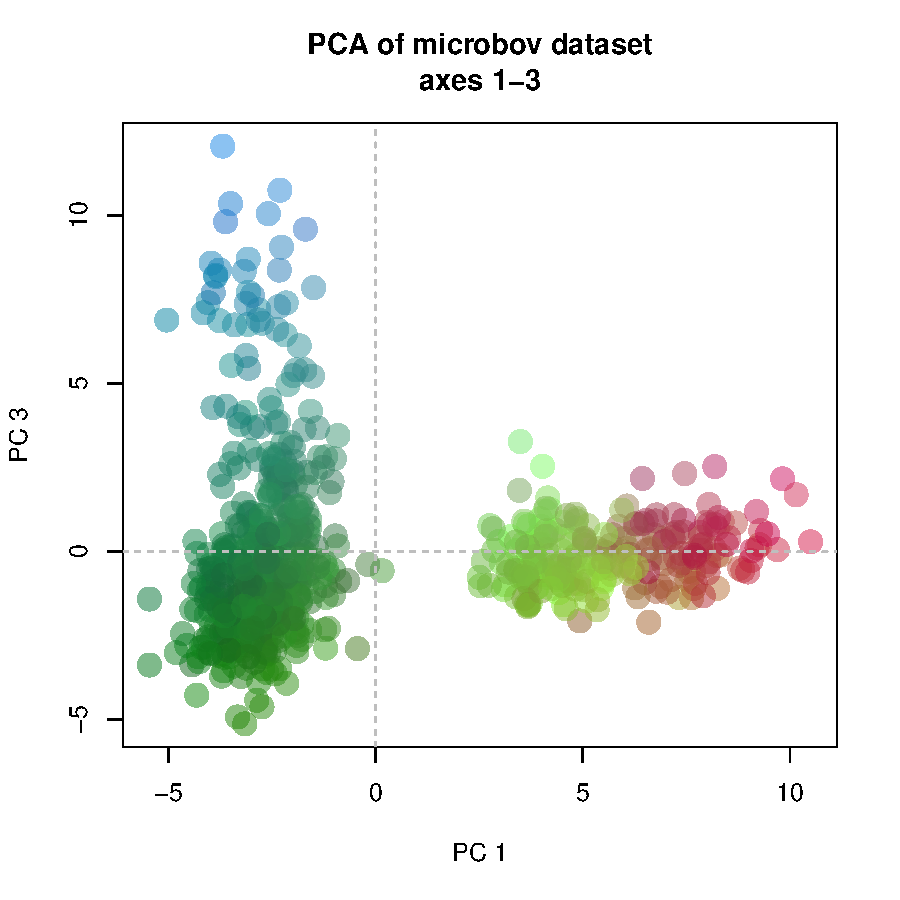
\includegraphics{figs/base-080}

\noindent The original value of the correlation between the distance matrices is represented by the
dot, while histograms represent permuted values (i.e., under the absence of spatial structure).
Significant spatial structure would therefore result in the original value being out of the
reference distribution.
Here, isolation by distance is clearly not significant.
\\


Let us provide another example using a dataset of individuals simulated under an IBD model:
\begin{Schunk}
\begin{Sinput}
> data(spcaIllus)
> x <- spcaIllus$dat2B
> Dgen <- dist(x$tab)
> Dgeo <- dist(other(x)$xy)
> ibd <- mantel.randtest(Dgen, Dgeo)
> ibd
\end{Sinput}
\begin{Soutput}
Monte-Carlo test
Call: mantel.randtest(m1 = Dgen, m2 = Dgeo)

Observation: 0.1267341 

Based on 999 replicates
Simulated p-value: 0.001 
Alternative hypothesis: greater 

      Std.Obs   Expectation      Variance 
 3.4917048386 -0.0009677967  0.0013375798 
\end{Soutput}
\end{Schunk}
\begin{Schunk}
\begin{Sinput}
> plot(ibd)
\end{Sinput}
\end{Schunk}
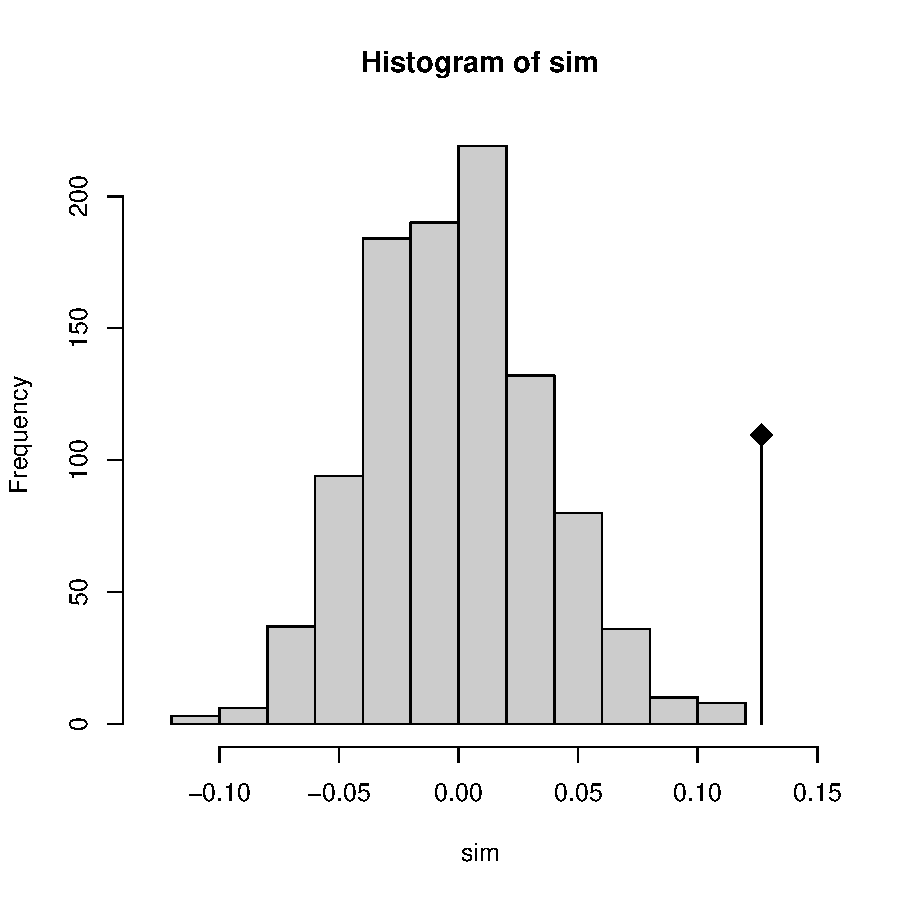
\includegraphics{figs/base-082}

\noindent This time there is a clear isolation by distance pattern.


% % % % % % % % % % % % % % % % % % % % %
\subsubsection{Cline or distant patches?}
% % % % % % % % % % % % % % % % % % % % %
The correlation between genetic and geographic distances can occur under a range of different
biological scenarios.
Classical IBD would result in continuous clines of genetic differentiation and cause such correlation.
However, distant and differentiated populations would also result in such a pattern.
These are slightly different processes and we would like to be able to disentangle them.
A very simple first approach is simply plotting both distances:
\begin{Schunk}
\begin{Sinput}
> plot(Dgeo, Dgen)
> abline(lm(Dgen ~ Dgeo), col = "red", lty = 2)
\end{Sinput}
\end{Schunk}
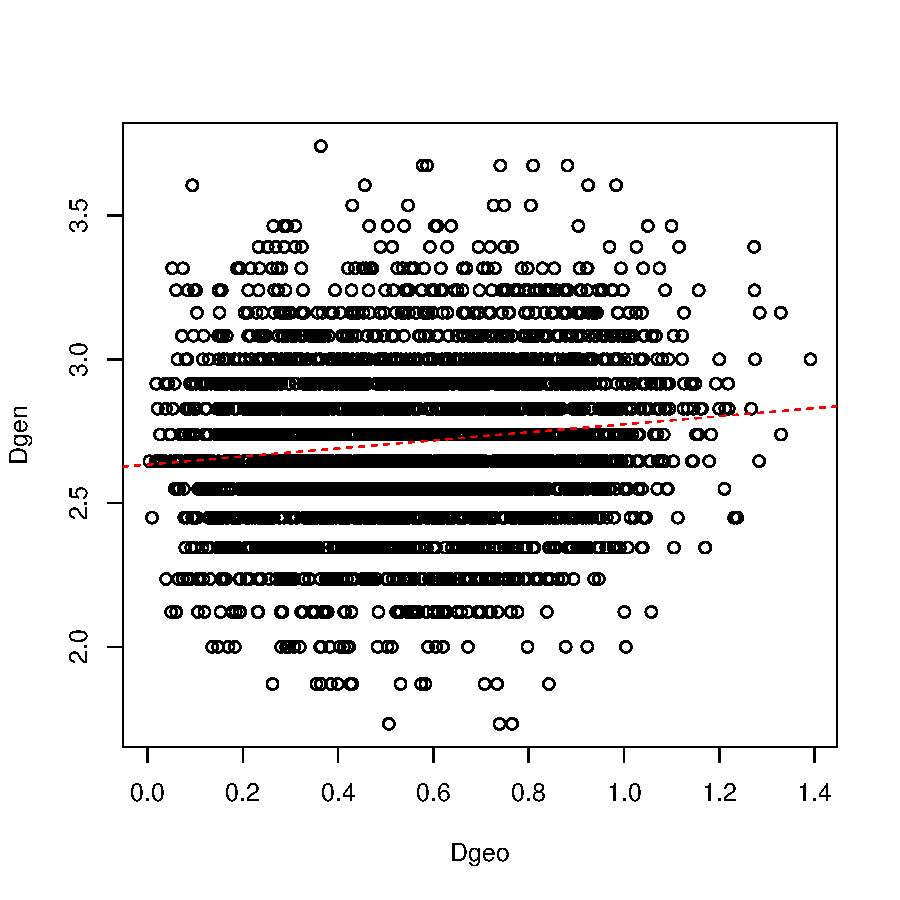
\includegraphics{figs/base-083}

\noindent Most of the time, simple scatterplots fail to provide a good picture of the data as the
density of points in the scatterplot is badly displayed.
Colors can be used to provide better (and prettier) plots.
Local density is measured using a 2-dimensional kernel density estimation (\texttt{kde2d}), and the
results are displayed using \texttt{image}; \texttt{colorRampPalette} is used to generate a
customized color palette:
\begin{Schunk}
\begin{Sinput}
> dens <- kde2d(Dgeo, Dgen, n = 300, lims = c(-0.1, 1.5, -0.5, 
+     4))
> myPal <- colorRampPalette(c("white", "blue", "gold", "orange", 
+     "red"))
> plot(Dgeo, Dgen, pch = 20, cex = 0.5)
> image(dens, col = transp(myPal(300), 0.7), add = TRUE)
> abline(lm(Dgen ~ Dgeo))
> title("Isolation by distance plot")
\end{Sinput}
\end{Schunk}
\begin{center}
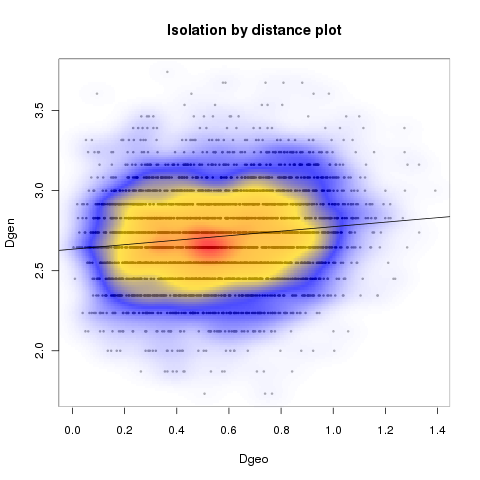
\includegraphics{figs/densIbd}
\end{center}

The scatterplot clearly shows one single consistent cloud of point, without discontinuities which
would have indicated patches.
This is reassuring, since the data were actually simulated under an IBD (continuous) model.




%%%%%%%%%%%%%%%%%%%%%%%%%%%%%%%%%%%%%%%%%%%%%%%%%%
\subsection{Using Monmonier's algorithm to define genetic boundaries}
%%%%%%%%%%%%%%%%%%%%%%%%%%%%%%%%%%%%%%%%%%%%%%%%%%
Monmonier's algorithm \cite{tj433} was originally designed to find boundaries of maximum differences between contiguous polygons of a tesselation.
As such, the method was basically used in geographical analysis.
More recently, \cite{np120} suggested that this algorithm could be employed to detect genetic boundaries among georeferecend genotypes (or populations).
This algorithm is implemented using a more general approach than the initial one in \textit{adegenet}.

Instead of using Voronoi tesselation as in original version, the functions \texttt{monmonier} and \texttt{optimize.monmonier} can handle various neighbouring graphs such as Delaunay triangulation, Gabriel's graph, Relative Neighbours graph, etc.
These graphs defined spatial connectivity among 'points' (genotypes or populations), any couple of points being neighbours (if connected) or not.
Another information is given by a set of markers which define genetic distances among these 'points'.
The aim of Monmonier's algorithm is to find the path through the strongest genetic distances between neighbours.
A more complete description of the principle of this algorithm will be found in the documentation of \texttt{monmonier}.
Indeed, the very purpose of this tutorial is simply to show how it can be used on genetic data.
\\

Let's take the example from the function's manpage and detail it.
The dataset used is \texttt{sim2pop}.

\begin{Schunk}
\begin{Sinput}
> data(sim2pop)
> sim2pop
\end{Sinput}
\begin{Soutput}
   #####################
   ### Genind object ### 
   #####################
- genotypes of individuals - 

S4 class:  genind
@call: old2new(object = sim2pop)

@tab:  130 x 241 matrix of genotypes

@ind.names: vector of  130 individual names
@loc.names: vector of  20 locus names
@loc.nall: number of alleles per locus
@loc.fac: locus factor for the  241 columns of @tab
@all.names: list of  20 components yielding allele names for each locus
@ploidy:  2
@type:  codom

Optionnal contents: 
@pop:  factor giving the population of each individual
@pop.names:  factor giving the population of each individual

@other: a list containing: xy 
\end{Soutput}
\begin{Sinput}
> summary(sim2pop$pop)
\end{Sinput}
\begin{Soutput}
P01 P02 
100  30 
\end{Soutput}
\begin{Sinput}
> temp <- sim2pop$pop
> levels(temp) <- c(3, 5)
> temp <- as.numeric(as.character(temp))
> plot(sim2pop$other$xy, pch = temp, cex = 1.5, xlab = "x", ylab = "y")
> legend("topright", leg = c("Pop A", "Pop B"), pch = c(3, 5))
\end{Sinput}
\end{Schunk}
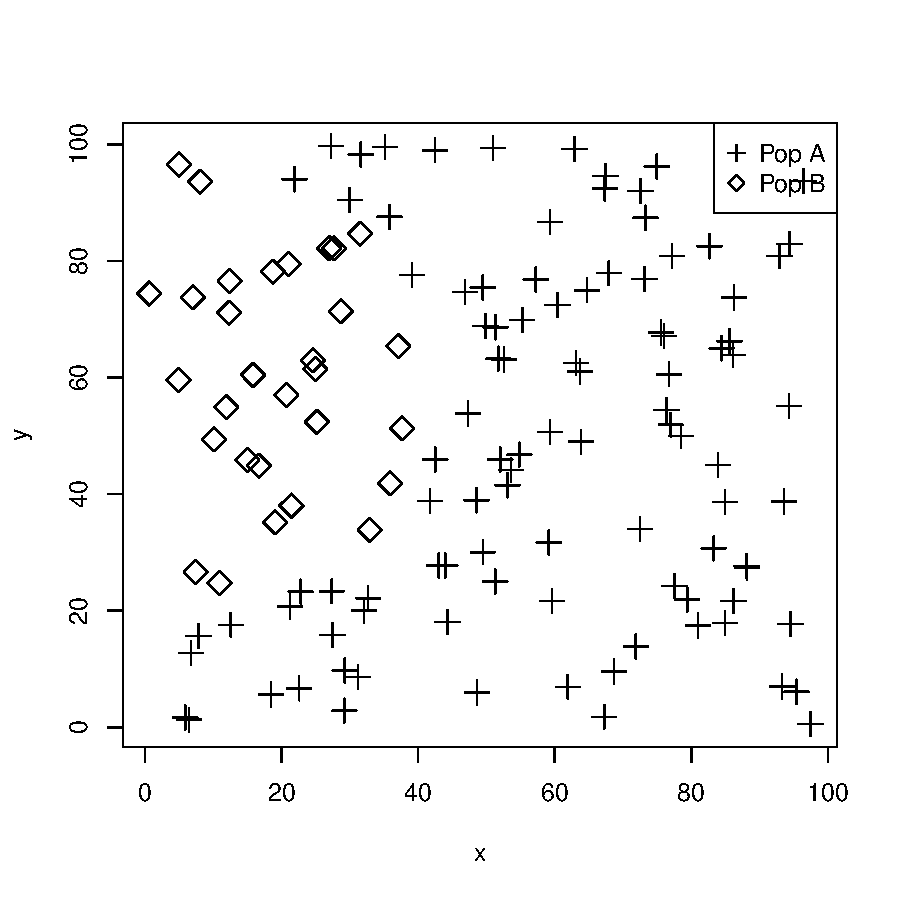
\includegraphics{figs/base-mon1}

There are two sampled populations in this dataset, with inequal sample sizes (100 and 30).
Twenty microsatellite-like loci are available for all genotypes (no missing data).
So, what do \texttt{monmonier} ask for?
\begin{Schunk}
\begin{Sinput}
> args(monmonier)
\end{Sinput}
\begin{Soutput}
function (xy, dist, cn, threshold = NULL, bd.length = NULL, nrun = 1, 
    skip.local.diff = rep(0, nrun), scanthres = is.null(threshold), 
    allowLoop = TRUE) 
NULL
\end{Soutput}
\end{Schunk}

\noindent The first argument (\texttt{xy}) is a matrix of geographic coordinates, already stored in \texttt{sim2pop}.
Next argument is an object of class \texttt{dist}, which is basically a distance matrix cut in half.
For now, we will use the classical Euclidean distance among alleles frequencies of genotypes.
This is obtained by:
\begin{Schunk}
\begin{Sinput}
> D <- dist(sim2pop$tab)
\end{Sinput}
\end{Schunk}

\noindent The next argument (\texttt{cn}) is a connection network.
As existing routines to build such networks are spread over several packages, the function \texttt{chooseCN} will help you choose one.
This is an interactive function, so difficult to demonstrate here (see \texttt{?chooseCN}).
Here we ask the function not to ask for a choice (\texttt{ask=FALSE}) and select the second type of graph which is the one of Gabriel (\texttt{type=2}).
\begin{Schunk}
\begin{Sinput}
> gab <- chooseCN(sim2pop$other$xy, ask = FALSE, type = 2)
\end{Sinput}
\begin{Soutput}
deldir 0.0-13 

     Please note: The process for determining duplicated points
     has changed from that used in version 0.0-9 (and previously).
\end{Soutput}
\end{Schunk}
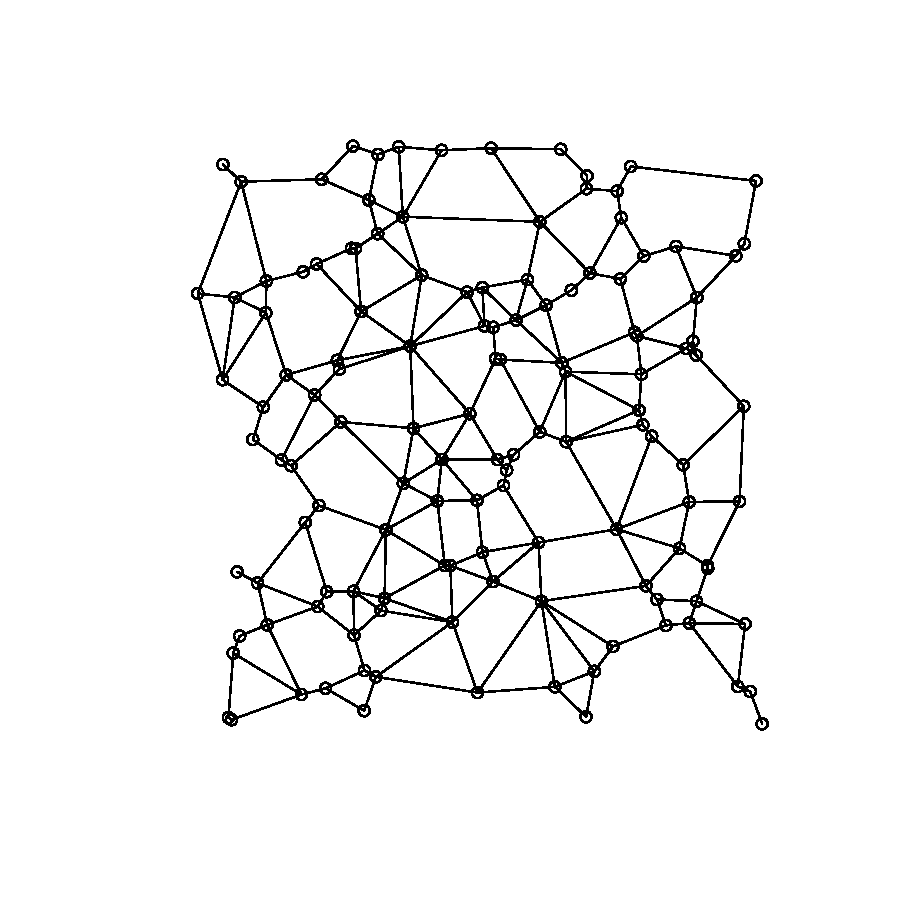
\includegraphics{figs/base-mon4}

\noindent The obtained network is automatically plotted by the function.
It seems we are now ready to proceed to the algorithm.
\begin{Schunk}
\begin{Sinput}
> mon1 <- monmonier(sim2pop$other$xy, D, gab)
\end{Sinput}
\end{Schunk}
\begin{center}
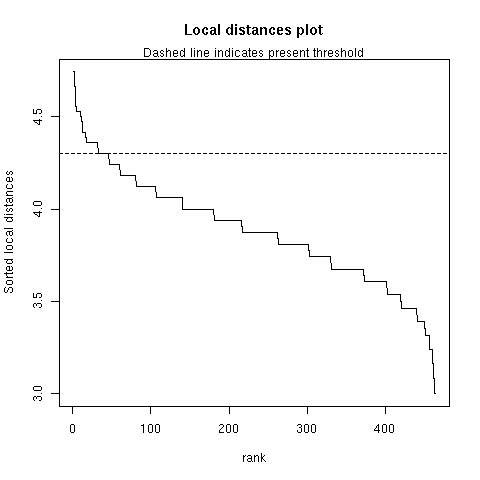
\includegraphics[width=.5\textwidth]{figs/monthres1.png}
\end{center}

\noindent This plot shows all local differences sorted in decreasing order.
The idea behind this is that a significant boundary would cause local differences to decrease abruptly after the boundary.This should be used to choose the \emph{threshold} difference for the algorithm to stop.
Here, no boundary is visible: we stop.
\\

Why do the algorithm fail to find a boundary?
Either because there is no genetic differentiation to be found, or because the signal differentiating both populations is too weak to overcome the random noise in genetic distances.
What is the $F_{st}$ between the two samples?
\begin{Schunk}
\begin{Sinput}
> pairwise.fst(sim2pop)
\end{Sinput}
\begin{Soutput}
           1
2 0.02343044
\end{Soutput}
\end{Schunk}

\noindent This value would be considered as very weak differentiation ($F_{ST}=0.023$).
Is it significant?
We can easily ellaborate a permutation test of this $F_{ST}$ value; to save computational time, we
use only a small number of replicates to generate $F_{ST}$ values in absence of population structure:
\begin{Schunk}
\begin{Sinput}
> replicate(10, pairwise.fst(sim2pop, pop = sample(pop(sim2pop))))
\end{Sinput}
\begin{Soutput}
 [1] 0.003484945 0.003764490 0.003314752 0.003239110 0.003821221 0.003562231
 [7] 0.004425530 0.005708968 0.003082894 0.003398615
\end{Soutput}
\end{Schunk}
$F_{ST}$ values in absence of population structure would be one order of magnitude lower (more
replicate would give a very low p-value --- just replace \texttt{10} by \texttt{200} in the above command).
In fact, the two samples are indeed genetically differentiated.
\\

Can Monmonier's algorithm find a boundary between the two populations?
Yes, if we get rid of the random noise.
This can be achieved using simple ordination method like Principal Coordinates Analysis.

\begin{Schunk}
\begin{Sinput}
> library(ade4)
> pco1 <- dudi.pco(D, scannf = FALSE, nf = 1)
> barplot(pco1$eig, main = "Eigenvalues")
\end{Sinput}
\end{Schunk}
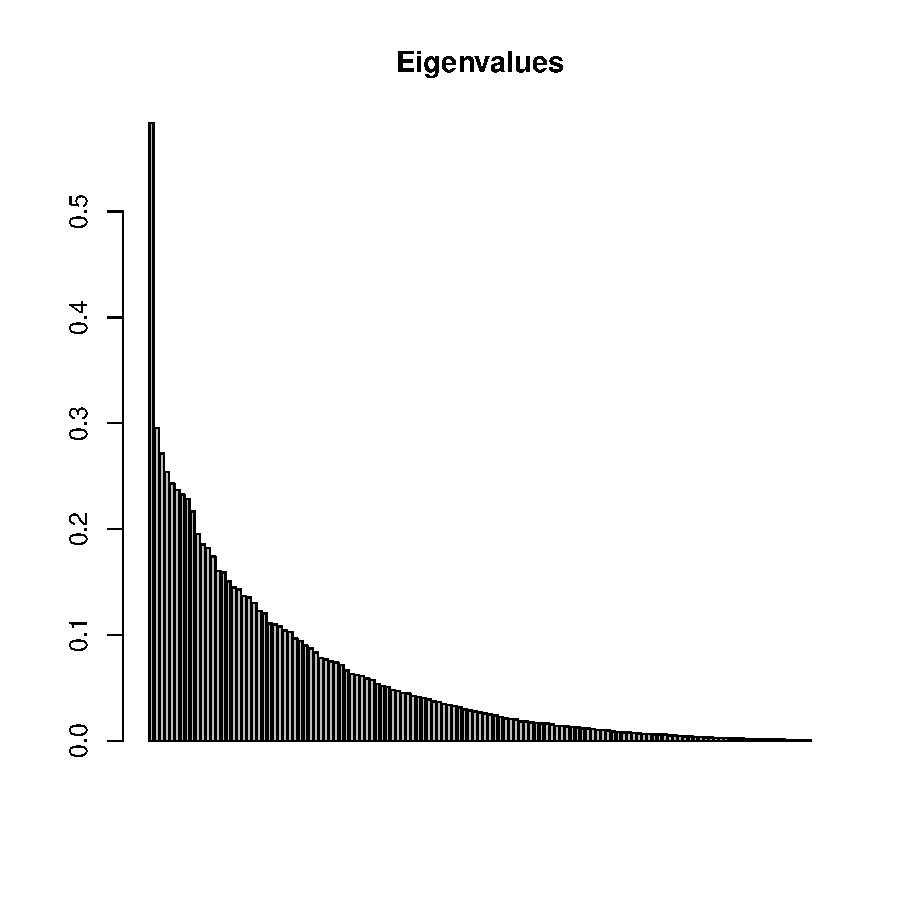
\includegraphics{figs/base-mon6}

\noindent We retain only the first eigenvalue.
The corresponding coordinates are used to redefine the genetic distances among genotypes.
The algorithm is then rerunned.
\begin{Schunk}
\begin{Sinput}
> D <- dist(pco1$li)
\end{Sinput}
\end{Schunk}
\begin{Schunk}
\begin{Sinput}
> mon1 <- monmonier(sim2pop$other$xy, D, gab)
\end{Sinput}
\end{Schunk}
\begin{center}
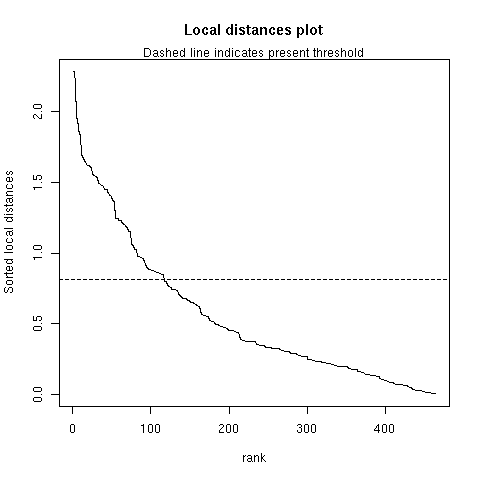
\includegraphics[width=.5\textwidth]{figs/monthres2.png}
\end{center}

\begin{Schunk}
\begin{Soutput}
###########################################################	
# List of paths of maximum differences between neighbours #	
#           Using a Monmonier based algorithm             #	
###########################################################

$call:monmonier(xy = sim2pop$other$xy, dist = D, cn = gab, scanthres = FALSE)

      # Object content #
Class:  monmonier
$nrun (number of successive runs):  1
$run1: run of the algorithm
$threshold (minimum difference between neighbours):  0.8154
$xy: spatial coordinates
$cn: connection network

      # Runs content #
# Run 1
# First direction
Class:  list
$path:
               x        y
Point_1 14.98299 93.81162

$values:
 2.281778
# Second direction
Class:  list
$path:
               x        y
Point_1 14.98299 93.81162
Point_2 30.74508 87.57724
Point_3 33.66093 86.14115
...

$values:
 2.281778 1.617905 1.95322 ...
\end{Soutput}
\end{Schunk}

\noindent This may take some time... but never more than five minutes on an 'ordinary' personnal computer.
The object \texttt{mon1} contains the whole information about the boundaries found.
As several boundaries can be seeked at the same time (argument \texttt{nrun}), you have to specify about which run and which direction you want to get informations (values of differences or path coordinates).
For instance:
\begin{Schunk}
\begin{Sinput}
> names(mon1)
\end{Sinput}
\begin{Soutput}
[1] "run1"      "nrun"      "threshold" "xy"        "cn"        "call"     
\end{Soutput}
\begin{Sinput}
> names(mon1$run1)
\end{Sinput}
\begin{Soutput}
[1] "dir1" "dir2"
\end{Soutput}
\begin{Sinput}
> mon1$run1$dir1
\end{Sinput}
\begin{Soutput}
$path
               x        y
Point_1 14.98299 93.81162

$values
[1] 2.281778
\end{Soutput}
\end{Schunk}

\noindent It can also be useful to identify which points are crossed
by the barrier; this can be done using \texttt{coords.monmonier}:
\begin{Schunk}
\begin{Sinput}
> coords.monmonier(mon1)
\end{Sinput}
\begin{Soutput}
$run1
$run1$dir1
            x.hw     y.hw first second
Point_1 14.98299 93.81162    11    125

$run1$dir2
             x.hw     y.hw first second
Point_1  14.98299 93.81162    11    125
Point_2  30.74508 87.57724    44    128
Point_3  33.66093 86.14115    20    128
Point_4  35.28914 81.12578    68    128
Point_5  33.85756 74.45492    68    117
Point_6  38.07622 71.47532    68    122
Point_7  41.97494 70.02783    35    122
Point_8  43.45812 67.12026    69    122
Point_9  42.20206 59.59613    22    122
Point_10 42.48613 52.55145    22    124
Point_11 40.08702 48.61795    13    124
Point_12 39.20791 43.89978    13    127
Point_13 38.81236 40.34516    62    127
Point_14 37.32112 36.35265    62    130
Point_15 37.96426 30.82105    94    130
Point_16 32.79703 28.00517    16    130
Point_17 30.12832 28.60376    85    130
Point_18 20.92496 29.21211    63    119
Point_19 16.05811 22.72600    61    126
Point_20 11.72524 21.15519    89    126
Point_21 10.18696 16.61536    74     89
\end{Soutput}
\end{Schunk}

\noindent The returned dataframe contains, in this order, the $x$ and
$y$ coordinates of the points of the barrier, and the identifiers of
the two 'parent' points, that is, the points whose barycenter is the
point of the barrier.

Finally, you can plot very simply the obtained boundary using the method \texttt{plot}:
\begin{Schunk}
\begin{Sinput}
> plot(mon1)
\end{Sinput}
\end{Schunk}
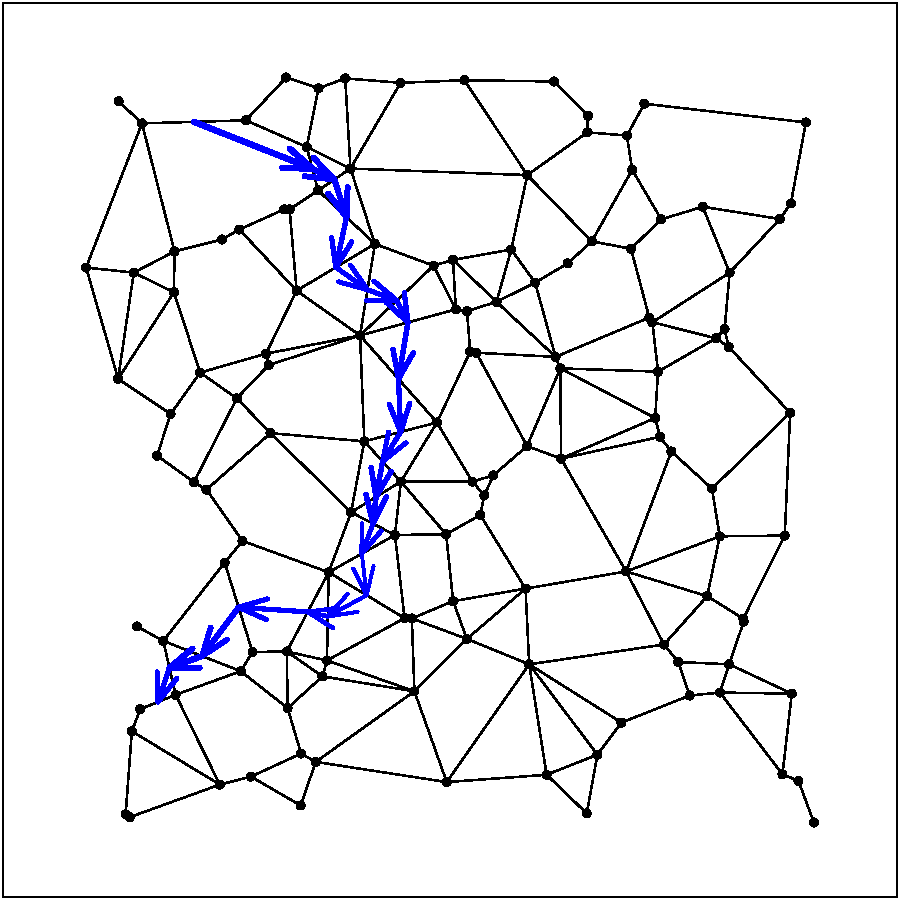
\includegraphics{figs/base-098}

\noindent see arguments in \texttt{?plot.monmonier} to customize this representation.
Last, we can compare the infered boundary with the actual distribution of populations:
\begin{Schunk}
\begin{Sinput}
> plot(mon1, add.arrows = FALSE, bwd = 8)
> temp <- sim2pop$pop
> levels(temp) <- c(3, 5)
> temp <- as.numeric(as.character(temp))
> points(sim2pop$other$xy, pch = temp, cex = 1.3)
> legend("topright", leg = c("Pop A", "Pop B"), pch = c(3, 5))
\end{Sinput}
\end{Schunk}
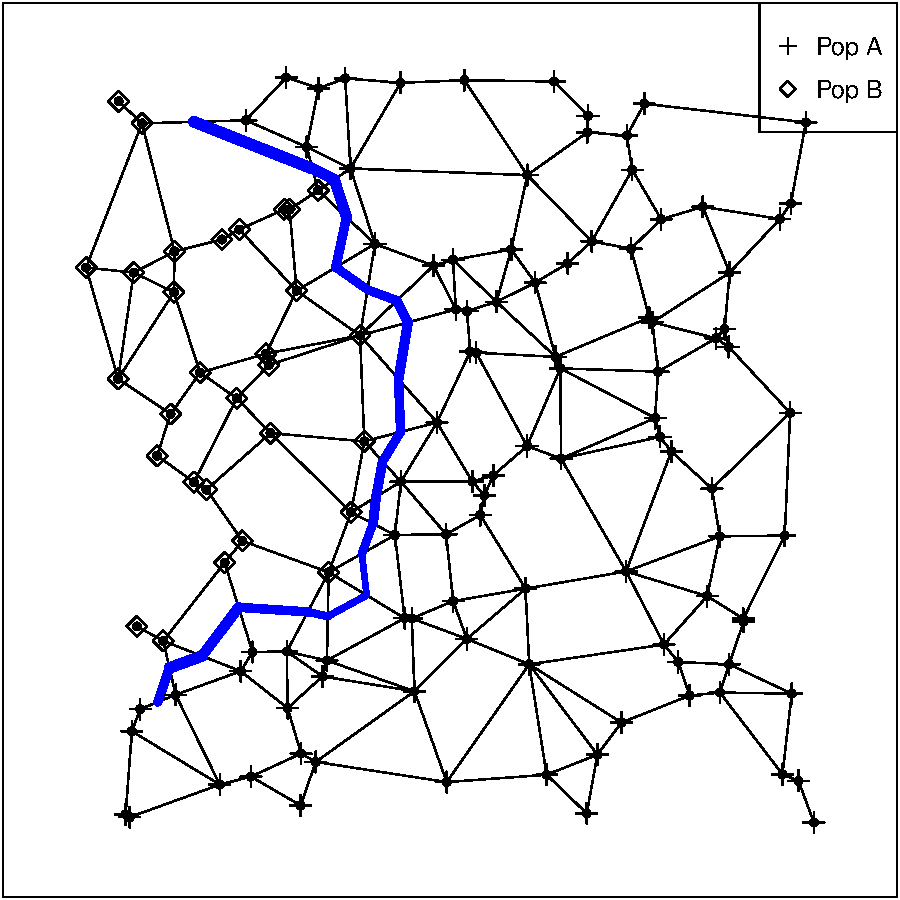
\includegraphics{figs/base-099}

\noindent Not too bad...




%%%%%%%%%%%%%%%%%%%%%%%%%%%%%%%%%%%%%%%%%%%%%%%%%%
%%%%%%%%%%%%%%%%%%%%%%%%%%%%%%%%%%%%%%%%%%%%%%%%%%
\section{Simulating hybridization}
%%%%%%%%%%%%%%%%%%%%%%%%%%%%%%%%%%%%%%%%%%%%%%%%%%
%%%%%%%%%%%%%%%%%%%%%%%%%%%%%%%%%%%%%%%%%%%%%%%%%%
The function \texttt{hybridize} allows to simulate hybridization between
individuals from two distinct genetic pools, or more broadly between
two \texttt{genind} objects.
Here, we use the example from the manpage of the function, to go a
little further.
Please have a look at the documentation, especially at the different
possible outputs (outputs for the software STRUCTURE is notably available).
\begin{Schunk}
\begin{Sinput}
> temp <- seppop(microbov)
> names(temp)
\end{Sinput}
\begin{Soutput}
 [1] "Borgou"          "Zebu"            "Lagunaire"       "NDama"          
 [5] "Somba"           "Aubrac"          "Bazadais"        "BlondeAquitaine"
 [9] "BretPieNoire"    "Charolais"       "Gascon"          "Limousin"       
[13] "MaineAnjou"      "Montbeliard"     "Salers"         
\end{Soutput}
\begin{Sinput}
> salers <- temp$Salers
> zebu <- temp$Zebu
> zebler <- hybridize(salers, zebu, n = 40, pop = "zebler")
\end{Sinput}
\end{Schunk}

\noindent A first generation (F1) of hybrids 'zebler' is obtained.
Is it possible to perform a backcross, say, with 'salers' population?
Yes, here it is:
\begin{Schunk}
\begin{Sinput}
> F2 <- hybridize(salers, zebler, n = 40)
> F3 <- hybridize(salers, F2, n = 40)
> F4 <- hybridize(salers, F3, n = 40)
\end{Sinput}
\end{Schunk}
Finally, note that despite this example shows hybridization between
diploid organisms, \texttt{hybridize} is not retrained to this case.
In fact, organisms with any even level of ploidy can be used, in which
case half of the genes is taken from each reference population.
Ultimately, more complex mating schemes could be
implemented... suggestion or (better) contributions are welcome!




\newpage
\begin{thebibliography}{9}

\bibitem{tjart05}
  Jombart, T. (2008) adegenet: a R package for the multivariate
  analysis of genetic markers. \textit{Bioinformatics} 24: 1403-1405.

\bibitem{np145}
  R Development Core Team (2011). R: A language and environment for
  statistical computing. R Foundation for Statistical Computing,
  Vienna, Austria. ISBN 3-900051-07-0.

\bibitem{tj548}
  Dray S and Dufour A-B (2007) The ade4 package: implementing the duality diagram for ecologists. \textit{Journal of Statistical Software} 22: 1-20.

\bibitem{tjart19}
  Jombart T, Devillard S and Balloux, F (2010).
  Discriminant analysis of principal components: a new method for the analysis of genetically structured populations.
  \textit{BMC Genetics} 11: 94.

\bibitem{tjart04}
  Jombart T, Devillard S, Dufour A-B and Pontier D (2008) Revealing cryptic spatial
  patterns in genetic variability by a new multivariate method.  \textit{Heredity} 101: 92-103.

\bibitem{tjart20}
  Jombart T, Eggo RM, Dodd PJ and Balloux F (2010) Reconstructing disease outbreaks from genetic
  data: a graph approach. \textit{Heredity} 106: 383-390.

\bibitem{tjart10}
  Jombart T, Pontier D and Dufour A-B (2009) Genetic markers in the playground of multivariate analysis.
  \textit{Heredity} 102: 330-341.

\bibitem{tj527}
  Paradis E, Claude J, and Strimmer K (2004) APE: analyses of phylogenetics and evolution in R language.
  \textit{Bioinformatics}: 20, 289-290.

\bibitem{np160}
  Charif D, and Lobry J (2007) SeqinR 1.0-2: a contributed package to the R project for statistical
  computing devoted to biological sequences retrieval and analysis. \textit{in} Structural approaches to sequence evolution: Molecules, networks, populations, \textit{Springer Verlag}, 207-232.

\bibitem{tj814}
  Nei M (1973) Analysis of gene diversity in subdivided populations. \textit{Proc Natl Acad Sci USA} 70: 3321-3323.


\bibitem{tj433}
  Monmonier M (1973) Maximum-difference barriers: an alternative numerical regionalization method. \textit{Geographical Analysis} 3: 245-261.

\bibitem{np120}
  Manni F, Guerard E and Heyer E (2004) Geographic patterns of (genetic, morphologic, linguistic)
  variation: how barriers can be detected by "Monmonier's algorithm". \textit{Human Biology} 76: 173-190.


\end{thebibliography}

\end{document}

